\documentclass{beamer}

\usepackage[backend=bibtex]{biblatex}
\bibliography{biblio.bib}


\usepackage{color}
%%to remove caption figure
\usepackage{caption}
\captionsetup[figure]{labelformat=empty}%
\usepackage{multimedia}
\usepackage{media9}
\usepackage{multicol}
\usepackage{graphicx}
\usepackage{caption}
\usepackage{subcaption}
\usetheme{default}

\AtBeginSection[]
  {
     \begin{frame}<beamer>
     \frametitle{Outline}
     \tableofcontents[currentsection]
     \end{frame}
  }

\addtobeamertemplate{navigation symbols}{}{%
    \usebeamerfont{footline}%
    \usebeamercolor[fg]{footline}%
    \hspace{1em}%
    \insertframenumber/\inserttotalframenumber
}

\title{Towards image-based cancer signatures from histopathology data}

%maybe add Supervisor\dfrac{•}{•}
\subtitle{First year report}

%\author{Naylor Peter}
\author[Naylor Peter]{Naylor Peter\\{\small Supervised by: T. Walter and F. Reyal}\\{\small Units: Center for Computational Biology and UMR900}}
\date{8th of June 2016}

\subject{THIS IS TRASH TRASH}

\AtBeginSubsection[]
{
  \begin{frame}<beamer>{Outline}
    \tableofcontents[currentsection,currentsubsection]
  \end{frame}
}

\titlegraphic{
\includegraphics[height=1.5cm]{Mines_ParisTech.png}~
	  
\includegraphics[height=1.5cm]{CURIE.jpg}~
	  
\includegraphics[height=0.7cm]{INSERM.jpg}}
\begin{document}

\begin{frame}
  \titlepage
\end{frame}

\begin{frame}{Outline}
  \tableofcontents
  % You might wish to add the option [pausesections]
\end{frame}

% Section and subsections will appear in the presentation overview
% and table of contents.
\section{Introduction}
\begin{frame}{Introduction}
Image data in biology or in medicine can be acquired in these settings:
\begin{itemize}
\item Fundamental research, through home brewed experiments: 

\begin{itemize}
\item[--] Microscopy data of cell cultures.
\item[--] In High content screening, many films (thousands) of experiments undergoing a different change.
\end{itemize}

\item In clinical practice: through practice of general medicine: 
\begin{itemize}
\item[--] Tissue scans, such as histopathology slide (PhD project)
\item[--] Photographs
\item[--] MRI scans
\item[--] Ultrasound \\
Etc
\end{itemize}

\end{itemize}

\end{frame}
\subsection{Masters/Side project}
%%% 3 slides
%%% About the master project
\begin{frame}{Time-lapse fluorescent microscopy data in the context of High Content Screening}
\textbf{Time-lapse microscopy}: Microscope image sequences, gives an accelerated view of the microscopic process. \\
\textbf{Fluorescent}:  In our case, after altering the experimental cells, certain proteins within the cell emit visible wave length. These proteins are used to highlight specific structures.
\begin{itemize}
\item H2B-eGFP is informative about the mitotic events.
\item PCNA-mcherry is informative about non mitotic events.
\end{itemize}

\begin{columns}[T] % align columns

\begin{column}{.45\textwidth}
\begin{figure}
\centering
\movie[autostart,loop,poster,width=\textwidth,showcontrols=false]{
\includegraphics[width=\textwidth]{defaultblack.jpg}}{Incenp.mp4}
\caption{Incenp}
\end{figure}
\end{column}

\begin{column}{.45\textwidth}
\begin{figure}
\centering
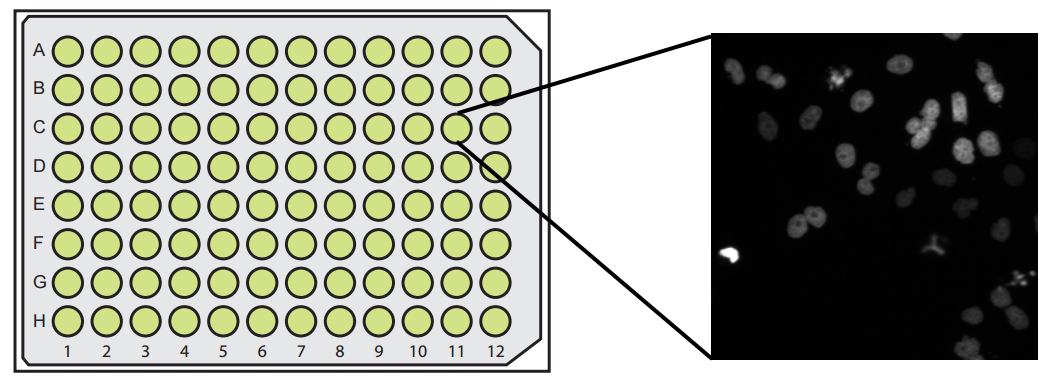
\includegraphics[width=\textwidth]{Images/plate_well.png}
\caption{High Content Screening}
\end{figure}
\end{column}
\end{columns}
\end{frame}


\begin{frame}{Recycling the MitoCheck project}
The mitocheck dataset is a unique dataset with a chromosome marker (H2B-eGFP). 200 000 filmed loss of function experiments. Can we used this data set to study the non-mitotic cell cycle phases? Idealy we would use a replication marker (PCNA-mcherry) but it is absent here.
\begin{figure}[!ht]
\centering
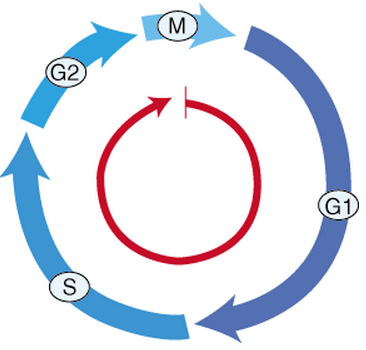
\includegraphics[width=0.3\textwidth]{Images/somaticcellcycle3.png}
\caption{Cell cycle}
\label{cellcycle}
\end{figure}
\end{frame}

\begin{frame}{The raw data}
\begin{columns}[T] % align columns
\begin{column}{.40\textwidth}
\begin{footnotesize}
\begin{figure}[!ht]
\centering
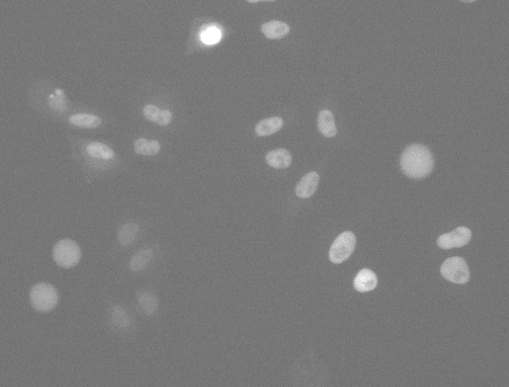
\includegraphics[width=0.50\textwidth]{Images/PCNA.png}
\caption{Data acquired by Michael Olma with the \texttt{PCNA} marker}
\label{PCNA_michael_olma}
\end{figure}
\begin{itemize}
\item Data set that helps us label the data.
\item HeLa cells stably expressing \texttt{PCNA} marker which is informative about the non-mitotic phases.
\end{itemize}
\end{footnotesize}
\end{column}%
\hfill%
\begin{column}{.56\textwidth}
\begin{footnotesize}
\begin{figure}[!ht]
\centering
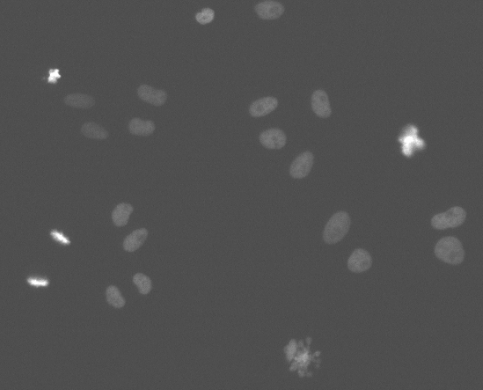
\includegraphics[width=0.38\textwidth]{Images/H2B.png}
\caption{Data acquired by Michael Olma with the \texttt{H2B} marker}
\label{H2B}
\end{figure}
\begin{itemize}
\item Data set from which we extract features for training purposes. 
\item Looking for paterns that help differenciate non-mitotic phases.
\item HeLa cells stably expressing \texttt{H2B} marker, informative about the mitotic phases.
\end{itemize}
\end{footnotesize}
\end{column}%
\end{columns}
\end{frame}

\begin{frame}{Extracting the data}

Using \textit{CellCognition}:
\begin{figure}[!ht]
\centering
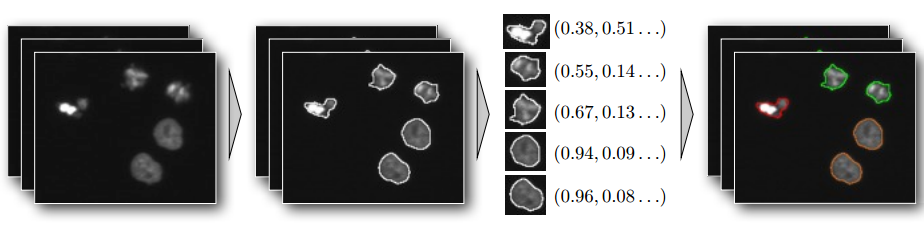
\includegraphics[width=\textwidth]{Images/features_extract.png}
\caption{\textit{CellCognition} steps for feature extraction}
\label{extract}
\end{figure}
\end{frame}

\begin{frame}{Results on the cell cycle phases length}
\begin{footnotesize}
To assess our predicition, we looked at different cell cycle phases length out of 234 trajectories:
\begin{table}[!ht]
\centering
\begin{tabular}{|c|c|c|c|}
  \hline
  Length of:  & Mean & Standard deviation & Number of trajectories \\
  \hline
\text{G1} & 7.13 & 3.8 & 159 \\
  \hline
\text{S}  & 6.28 & 2.9 & 124 \\
  \hline
\text{G2} & 3.17 & 1.4 & 124 \\
  \hline
\text{Cell Cycle} & 16.7 & 4.1 & 124 \\
  \hline 
\end{tabular} 
  \caption{On Michael Olma set with the PCNA channel, our "ground truth"}
\end{table}
\begin{table}[!ht]
\begin{tabular}{|c|c|c|c|}
  \hline
  Length of:  & Mean & Standard deviation & Number of trajectories \\
  \hline
\text{G1} & 6.92 & 3.6 & 164 \\
  \hline
\text{S}  & 8.30 & 3.1 & 102 \\
  \hline
\text{G2} & 1.77 & 2.2 & 102 \\
  \hline
\text{Cell Cycle} & 17.1 & 2.1 & 102 \\
  \hline 
\end{tabular} 
  \caption{On Michael Olma set with the H2B channel}
\end{table}
\end{footnotesize}
\end{frame}



\subsection{Cancer Research}
%%% 2 frames approx
%Here I will be talking about cancer and why cancer research is important
\begin{frame}{Cancer research}
\begin{enumerate}
\item Cancer is a disease of the genome. \\ 
In the early 2000, first sequencing of the human genome.
\item Cancer is a very heterogeneous disease. 2 breast cancers can be totally different on a molecular basis. This disease is highly variable in many aspects, we therefore saw the emergence of personalized medicine. 
\item The clinical motivation for cancer research are: profiling each type of tumor, in terms of molecular subtype and prognostic in order features. On the long run this will lead to a better understanding, diagnostic, prognostic, ...
\end{enumerate}
\end{frame}

\begin{frame}{Why image based features in cancer research}
\begin{itemize}
\item In clinical practice, one looks at the available image data to give a treatment. 
\item Differently, in clinical research, one studies the images to infer properties.
\item Finding correspondence/correlations between genes and phenotypic information. 
\item Highly relevant data can be found. \\
\begin{itemize}
\item We can cross protein localization microscopy with loss-of-function experiment.
\item You access response to disease information, lymphocyte responses to tumor expansion. Different type of information, spatial repartition, neighbouring information, density, ..
\item Correcting noisy molecular data, mutation data will be mixture of healthy cells, cancerous cells, lymphocytes,...
\end{itemize}
\end{itemize}
\end{frame}



\section{Phd Subject}
%Here I will talk about my phd subject
%%% 3 frames approx

\begin{frame}{Histopathology: microscopic examination of tissue}
Different procedure of histopathology in breast cancer.
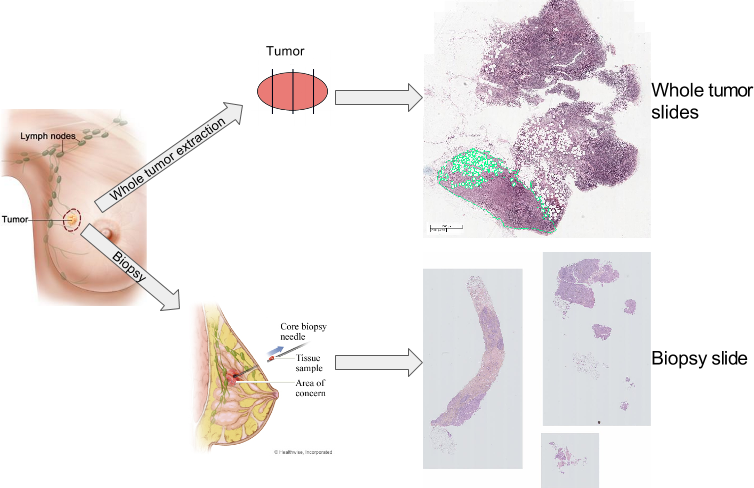
\includegraphics[width=\textwidth]{SlidePreparation.png}
\end{frame}
\begin{frame}{PhD pipeline}
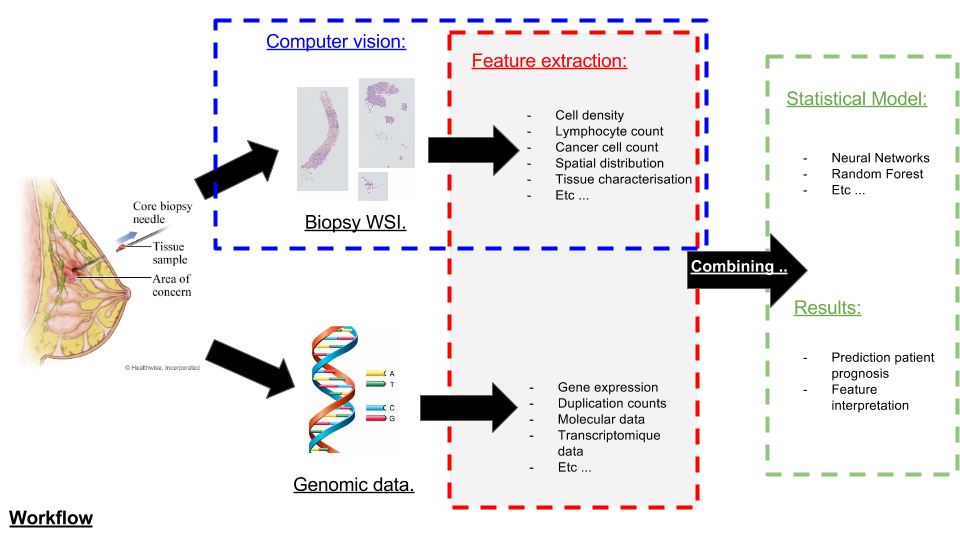
\includegraphics[width=\textwidth]{Workflow_overview.png}
\end{frame}
\begin{frame}{Main focus}
 Extracting relevant features at the cellular and tissue
level. \\
\textbf{Cellular level:}
\begin{itemize}
\item Segmentation at the cellular level. 
\item Classification of nuclei type: Lymphocyte, cancerous cell, normal cell, ...
\item Classification of nuclei state: Cell undergoing mitotic event, dead cell, ...
\end{itemize}

\textbf{Tissue level:}
\begin{itemize}
\item Segmentation at the tissue level.
\item Classification into regions: tumor,
stromal and necrotic. \\
Information at the cellular level could be used to help/correct prediction.
\end{itemize}

Main issue: As we wish this to be easily reproducible, the key problem is the segmentation.
\end{frame}

\begin{frame}{Application to two datasets}
\begin{enumerate}
\item 208 slides from an unpublished study on breast
cancer, a special type of very aggressive breast cancer  \\
\emph{Focus: treatment response to chemotherapy}.
\item 198
slides from a recently published study on bladder cancer \footfullcite{biton2014independent}.
\emph{Focus: Correlation between histopathology features with the
molecularly defined subgroups.}
\end{enumerate}
\end{frame} 



\begin{frame}{Difficulties}
%\begin{figure}[!ht]
%\centering
%\begin{subfigure}{.3\textwidth}
%  \centering
%  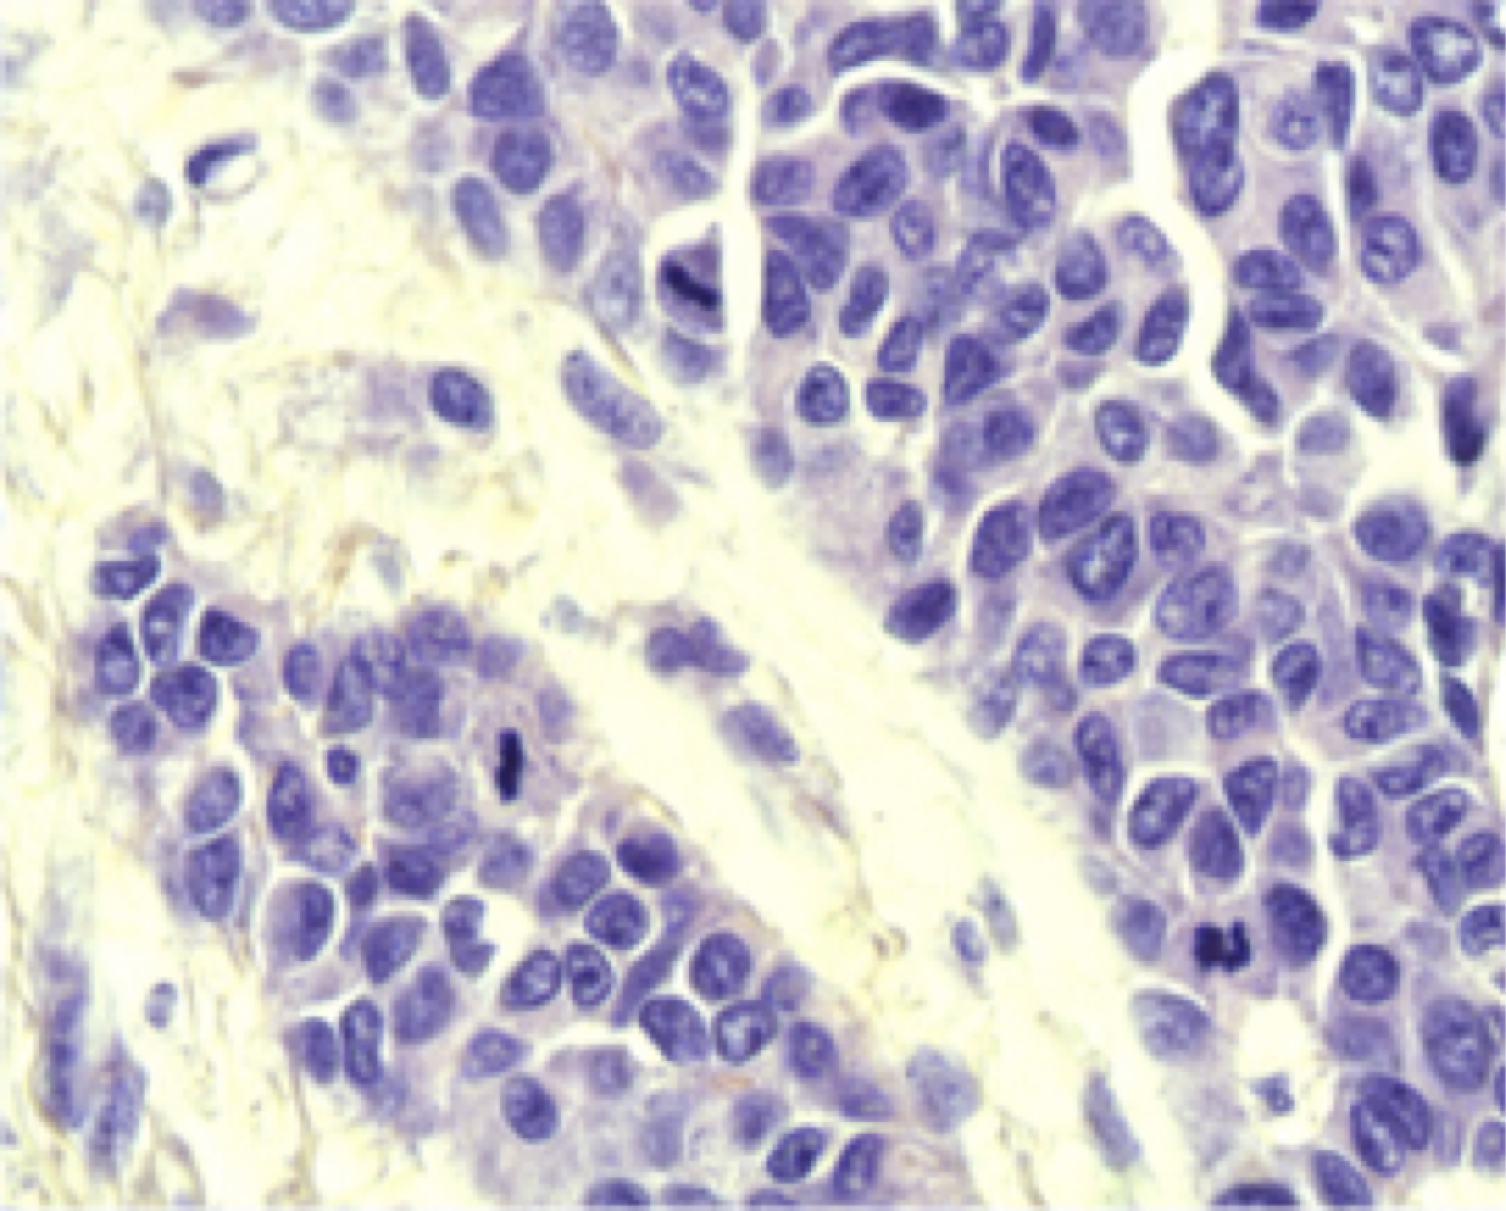
\includegraphics[height=4cm]{histo1.png}
%  \caption{}
%  \label{fig:sub1}
%\end{subfigure}%
%~
%\begin{subfigure}{.3\textwidth}
%  \centering
%  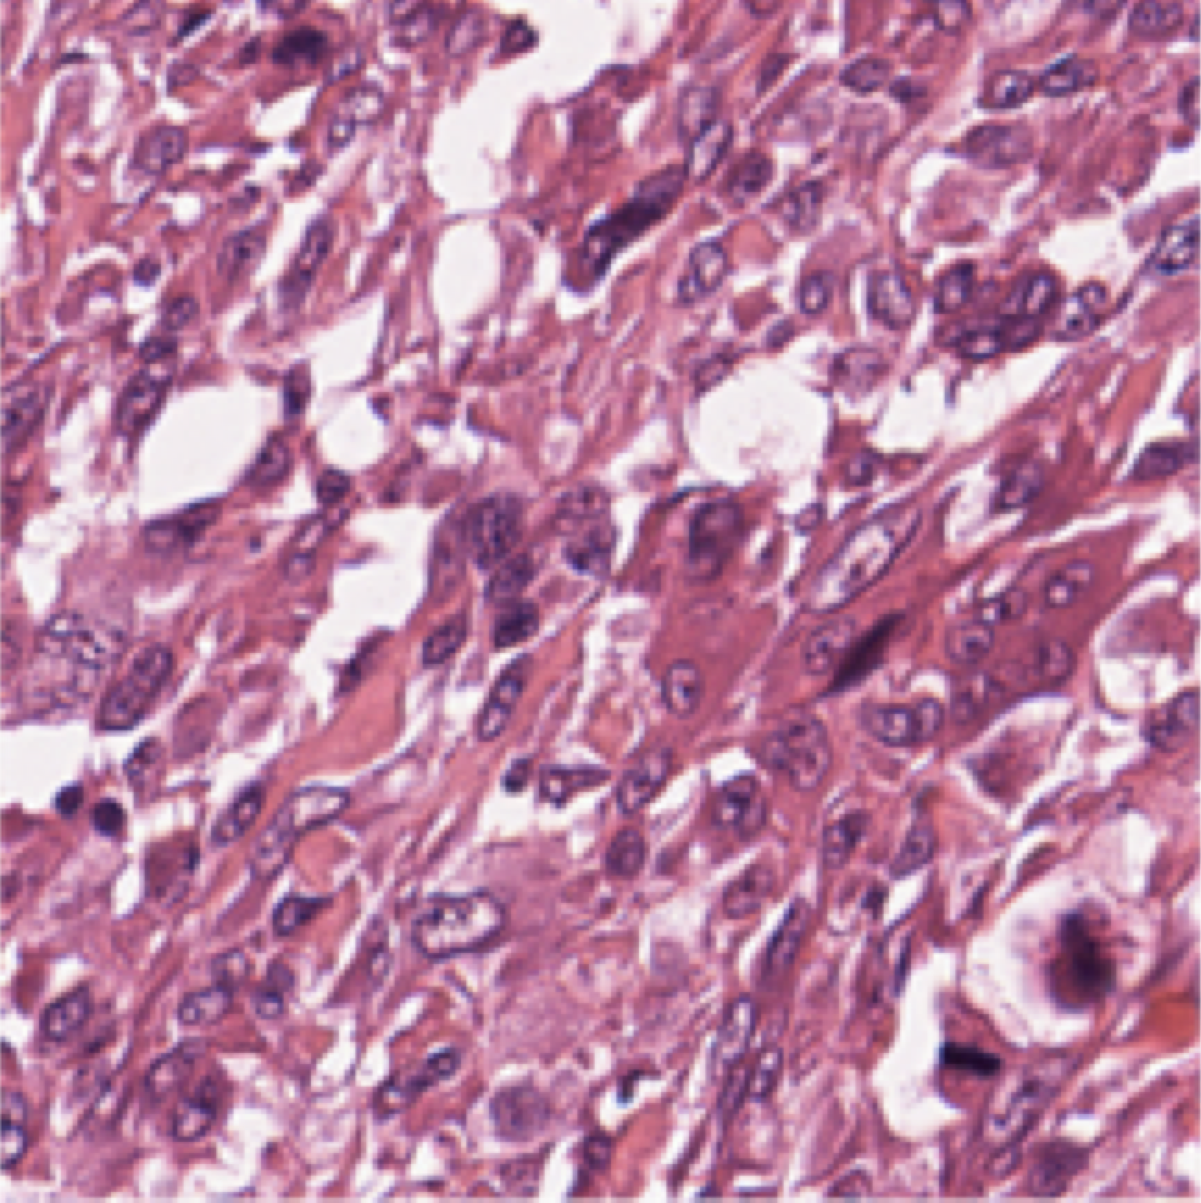
\includegraphics[height=4cm]{histo2.png}
%  \caption{}
%  \label{fig:sub2}
%\end{subfigure}
%~
%\begin{subfigure}{.3\textwidth}
%  \centering
%  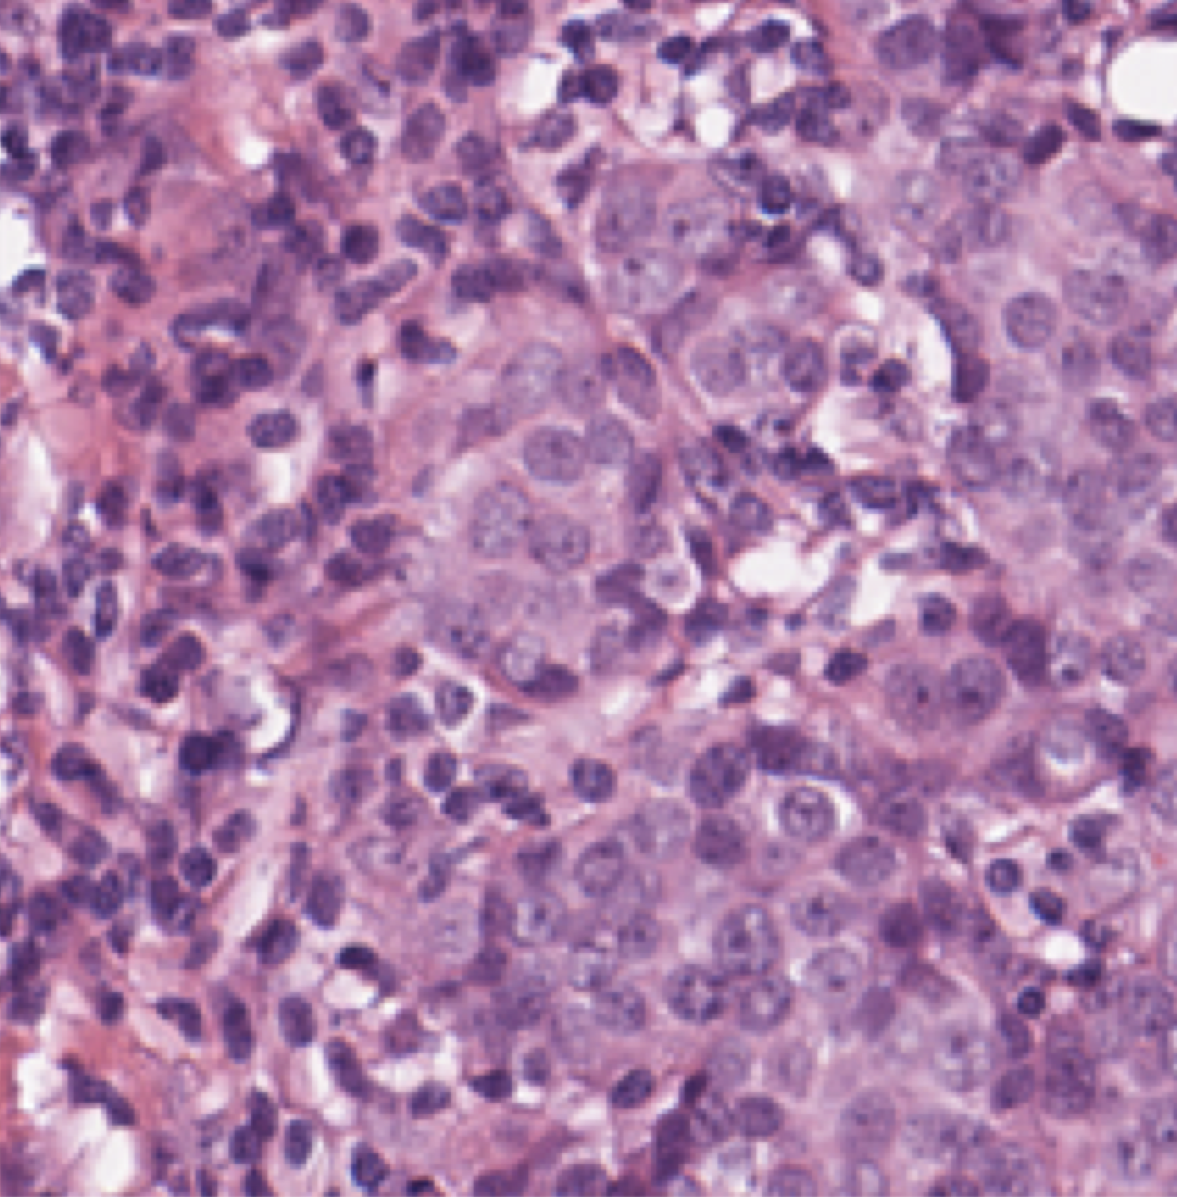
\includegraphics[height=4cm]{histo3.png}
%  \caption{}
%  \label{fig:sub3}
%\end{subfigure}
%\caption{Tissue sections with standard Haematoxylin and Eosin staining.}
%\label{fig:example_histopath}
%\end{figure}

\begin{columns}[T] % align columns
\begin{column}{.3\textwidth}
\begin{figure}[!ht]
\centering
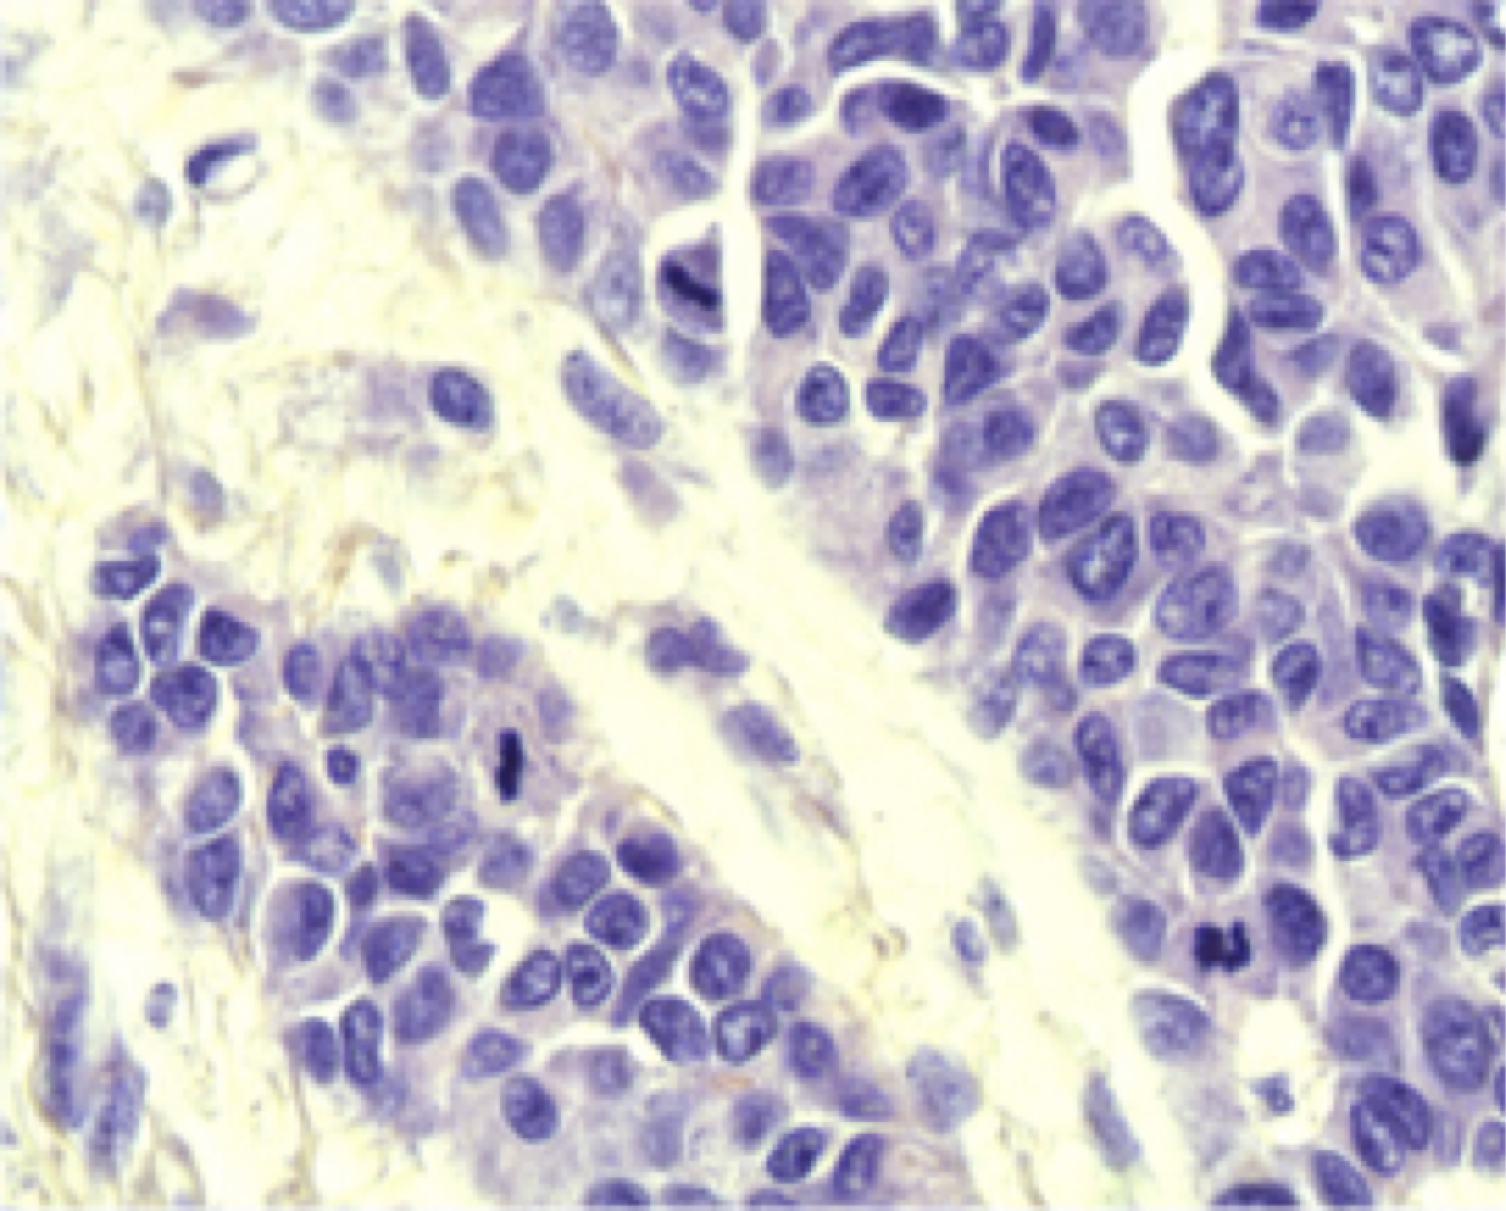
\includegraphics[width=\textwidth]{histo1.png}
%\caption{}
\label{}
\end{figure}
\end{column}%
\hfill%
\begin{column}{.3\textwidth}
\begin{figure}[!ht]
\centering
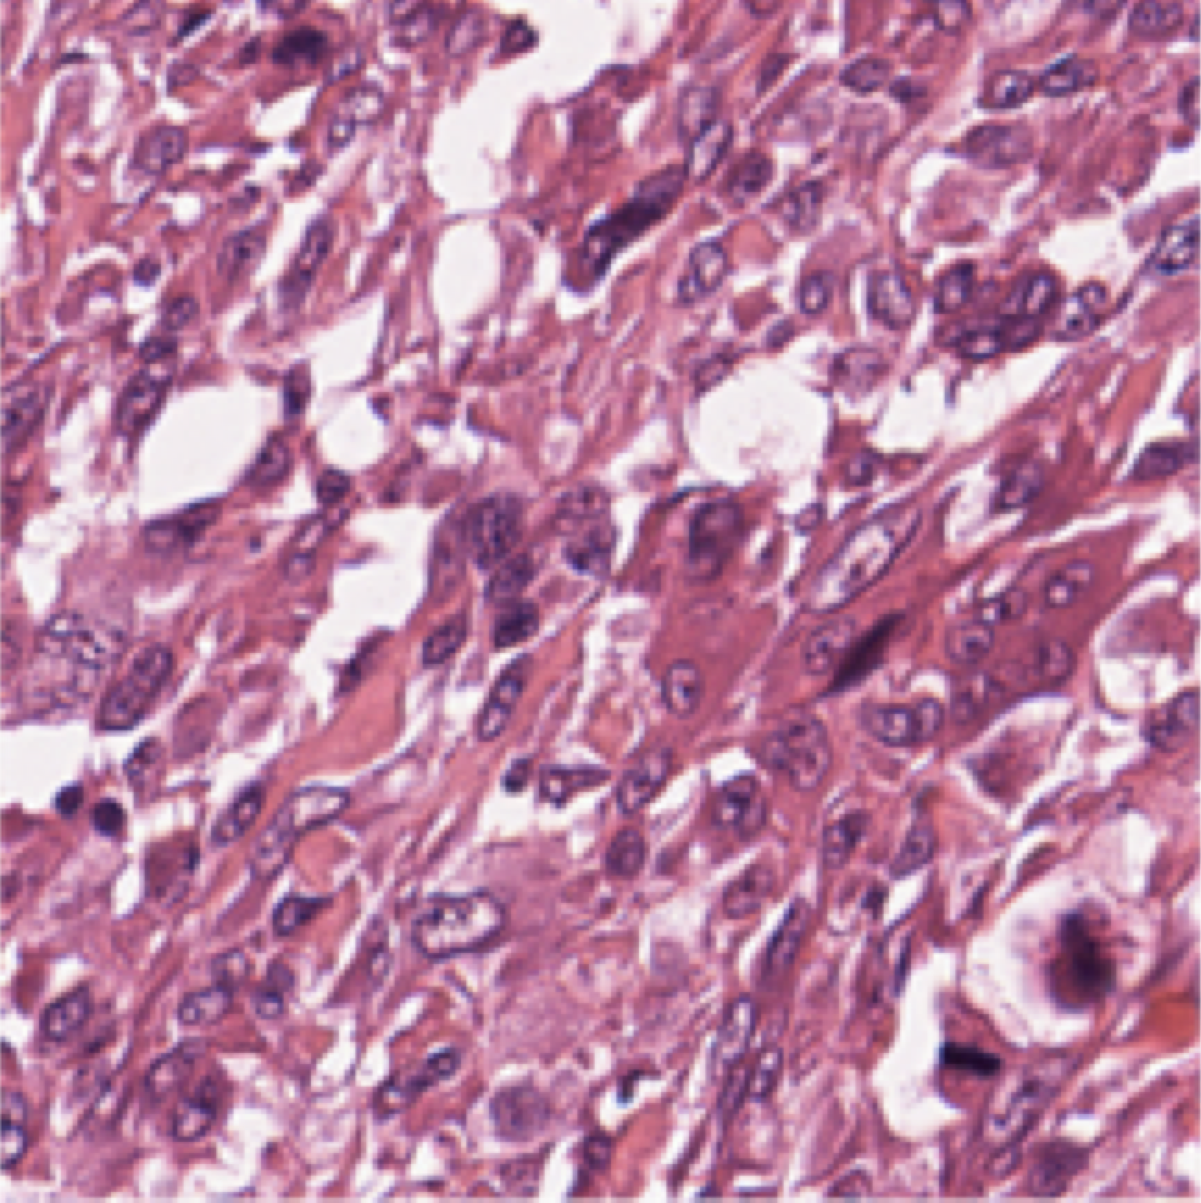
\includegraphics[width=\textwidth]{histo2.png}
%\caption{}
\label{}
\end{figure}
\end{column}%
\hfill%
\begin{column}{.3\textwidth}
\begin{figure}[!ht]
\centering
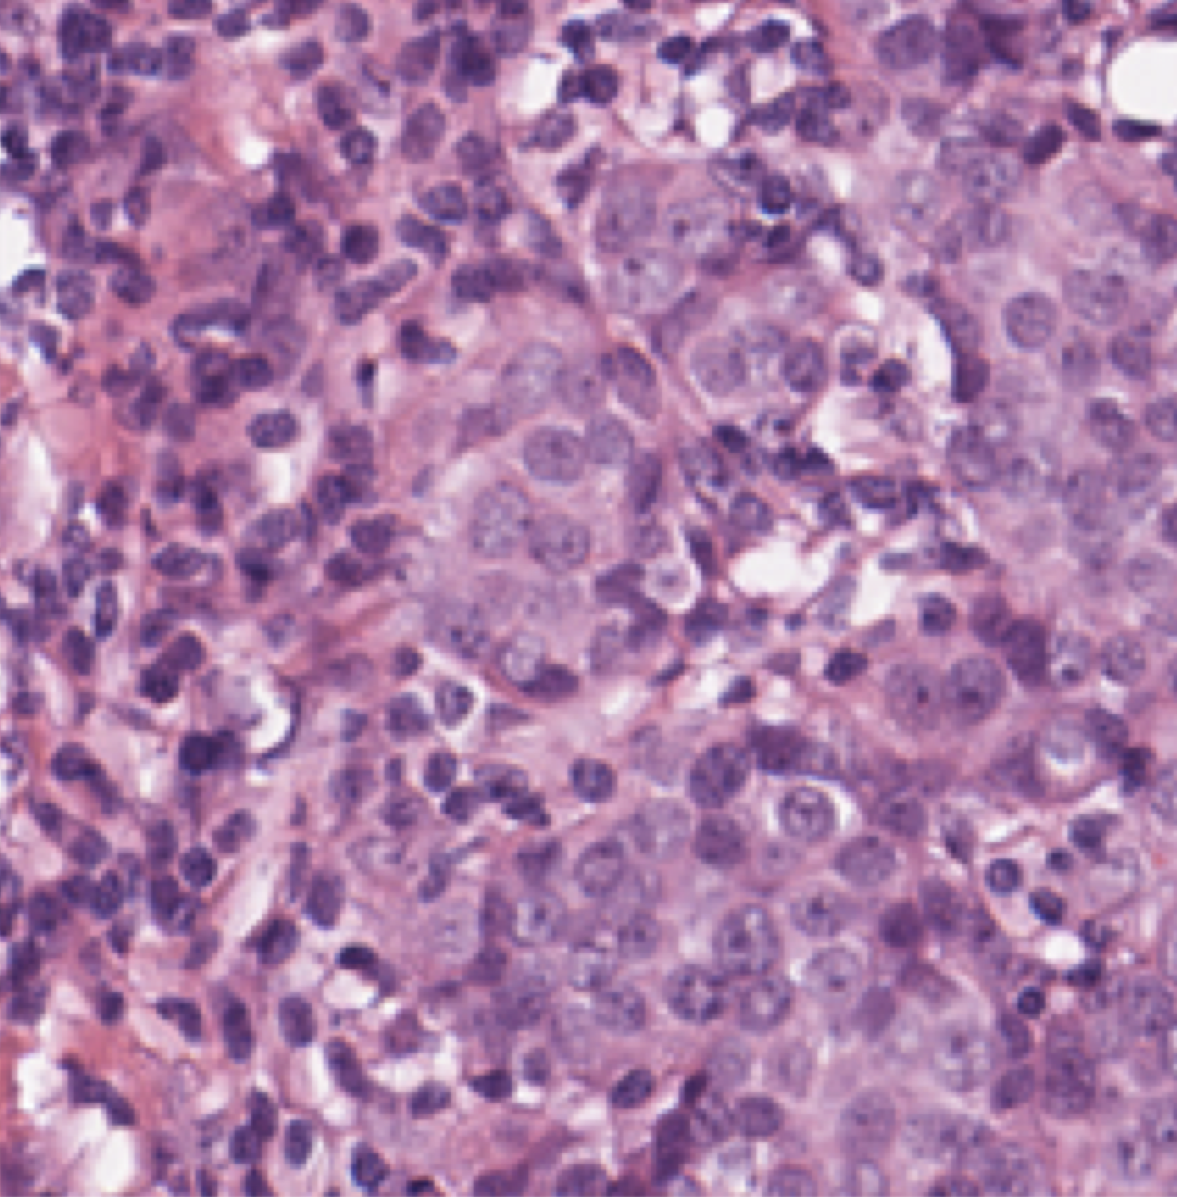
\includegraphics[width=\textwidth]{histo3.png}
%\caption{}
\label{}
\end{figure}
\end{column}%
\end{columns}
{\centering \textit{Tissue sections with standard Haematoxylin and Eosin staining}} 
\begin{itemize}
\item [--] High variability in staining.
\item [--] High variability in tissue objects.
\item [--] Difficult segmentation task. 
\end{itemize}


\end{frame}


\begin{frame}{Large image files: tiled tiff format}
One individual slide can be up to $50 GB$, uncompressed.
\begin{columns}[T] % align columns
\begin{column}{.3\textwidth}
\begin{figure}[!ht]
\centering
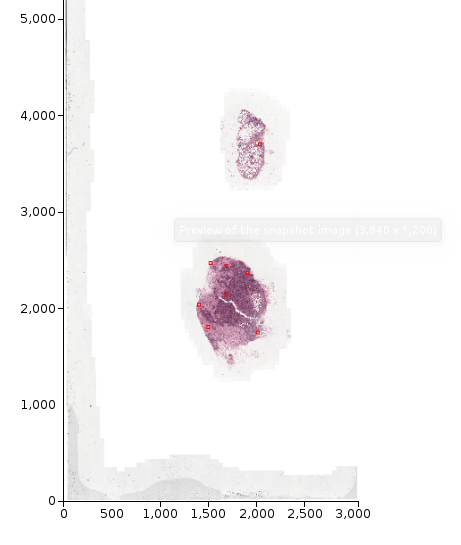
\includegraphics[width=\textwidth]{Tumor_31.png}
\caption{Tumor 31}
\textit{7000 x 3500, resolution 6}
\label{}
\end{figure}
\end{column}%
\hfill%
\begin{column}{.3\textwidth}
\begin{figure}[!ht]
\centering
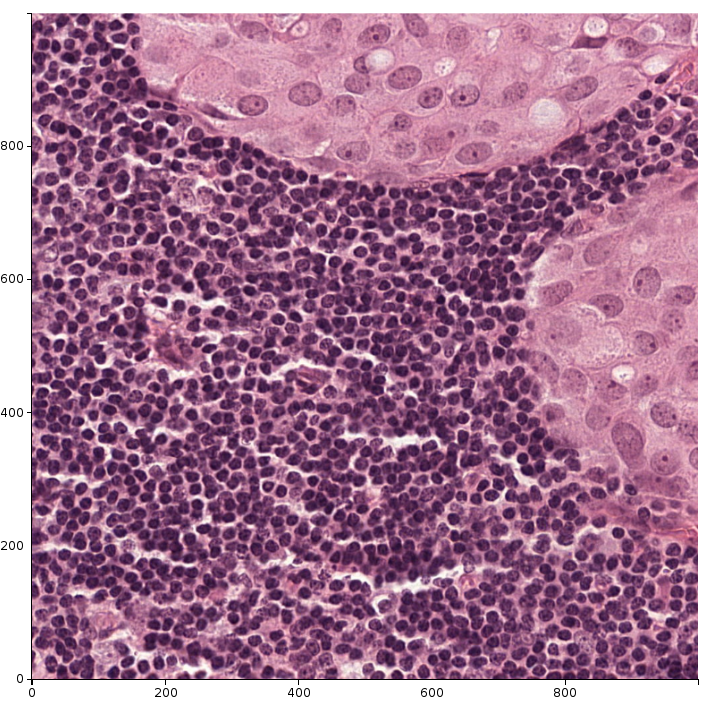
\includegraphics[width=\textwidth]{Tumor_31_res0.png}
\caption{Sub-image of Tumor 31, highest resolution}
\textit{1000 x 1000, resolution 0}
\label{}
\end{figure}
\end{column}%
\hfill%
\begin{column}{.3\textwidth}
\begin{figure}[!ht]
\centering
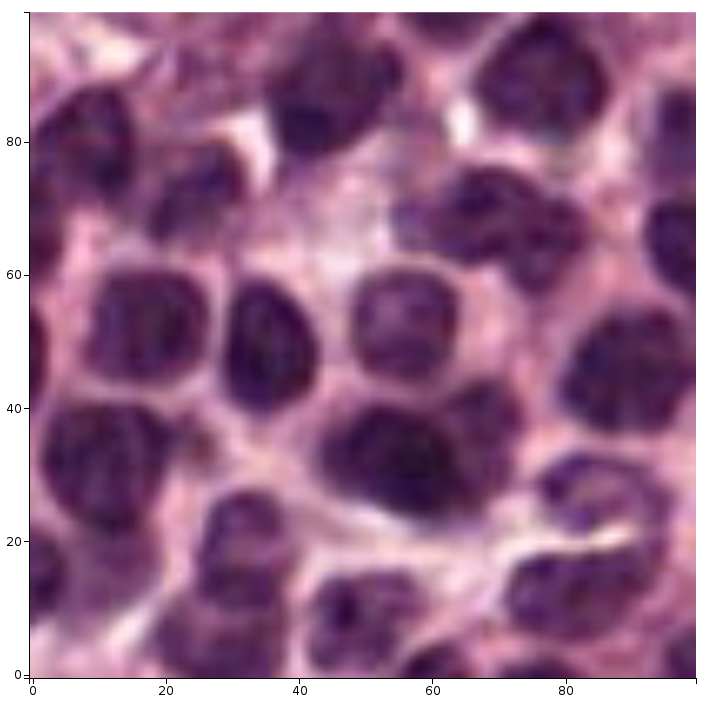
\includegraphics[width=\textwidth]{Tumor_31_res0_zoom.png}
\caption{Sub-image of Tumor 31, highest resolution (zoom)}
\textit{100 x 100, resolution 0}
\label{}
\end{figure}
\end{column}%
%\begin{column}{.25\textwidth}
%\begin{figure}[!ht]
%\centering
%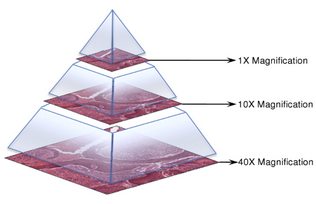
\includegraphics[width=\textwidth ,height=4cm]{pyramid.png}
%\caption{Pyramid data structure}
%\textit{Between 8 and 10 different resolutions}
%\label{}
%\end{figure}
%\end{column}
\end{columns}

%\begin{figure}[!ht]
%\centering
%\begin{subfigure}{.25\textwidth}
%  \centering
%  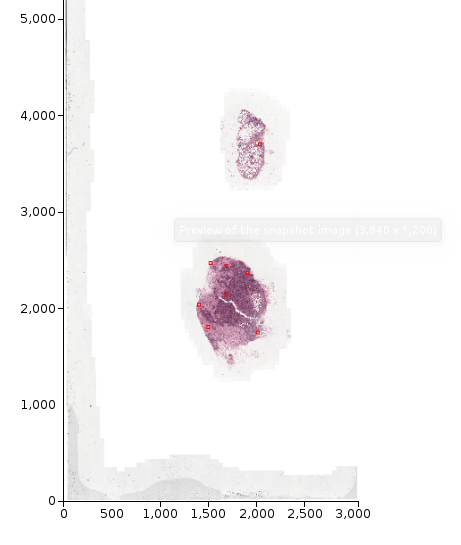
\includegraphics[width=\textwidth]{Tumor_31.png}
%  \caption{}
%  \label{fig:sub1}
%\end{subfigure}%
%~
%\begin{subfigure}{.25\textwidth}
%  \centering
%  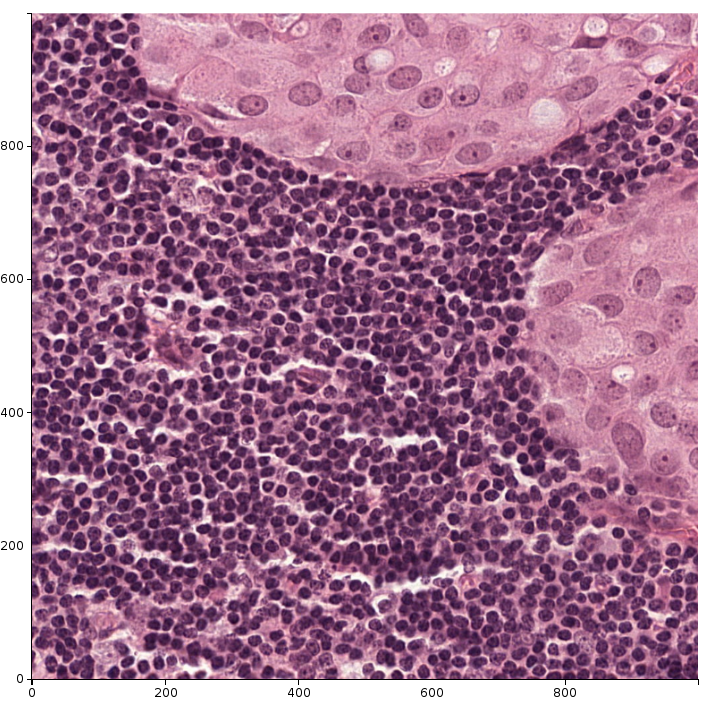
\includegraphics[width=\textwidth]{Tumor_31_res0.png}
%  \caption{}
%  \label{fig:sub2}
%\end{subfigure}
%~
%\begin{subfigure}{.25\textwidth}
%  \centering
%  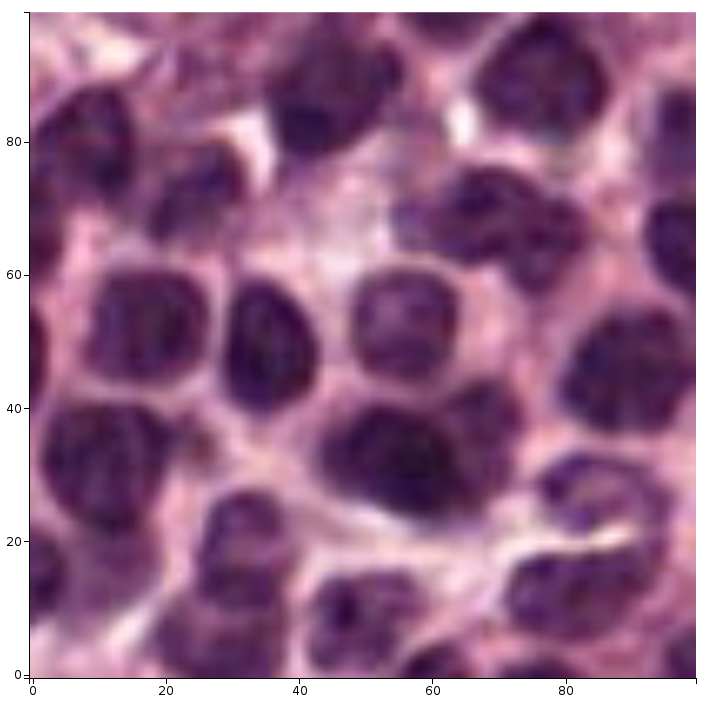
\includegraphics[width=\textwidth]{Tumor_31_res0_zoom.png}
%  \caption{}
%  \label{fig:sub3}
%\end{subfigure}
%~
%\begin{subfigure}{.25\textwidth}
%  \centering
%  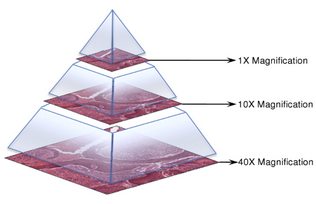
\includegraphics[width=\textwidth]{pyramid.png}
%  \caption{}
%  \label{fig:sub3}
%\end{subfigure}
%\caption{Tissue sections with standard Haematoxylin and Eosin staining.}
%\label{fig:example_histopath}
%\end{figure}

\end{frame}


\section{Tissue segmentation}
%% I will talk about the challenge, challenging work, novel features, annotated data
%% approx 6 slides
\begin{frame}{Camelyon2016}

\begin{columns}[T] % align columns
\begin{column}{.7\textwidth}
In many machine learning tasks, annotated data is very expensive. They often require experts and these task are long, tedious and prone to manual errors. Camelyon2016 provides:
\begin{itemize}
\item Over $500 GB$ of histopathology slides. (400 slides)
\item 270 fully annotated slides, for metastasis detection.
\item First experience with:
\begin{itemize}
\item [--] Histopathology data
\item [--] Computer vision
\item [--] Dealing with huge databases (clusters of computers)
\end{itemize} 
\end{itemize}
Work in collaboration with V. Machairas, E. Decenciere and T. Walter.
\end{column}%
\hfill%
\begin{column}{.3\textwidth}
\begin{figure}[!ht]
\centering

\includegraphics[width=1.3\textwidth]{Camelyon16.png}
\caption{Official logo}
\label{}
\end{figure}
\end{column}%
\end{columns}
\end{frame}

\begin{frame}{Pixel based classifier}
\textcolor{red}{Finding metastasis regions:}\\
Each pixel, will be considered metastasis if it belongs to a metastasis region. \\
Model: Modified random forest, each trees see a unique part of the data set. \\

\textcolor{red}{Cross-validation/evaluation:} \\
One slide out scheme.
\end{frame}

\begin{frame}{Work pipeline}
\begin{figure}[!ht]
\centering
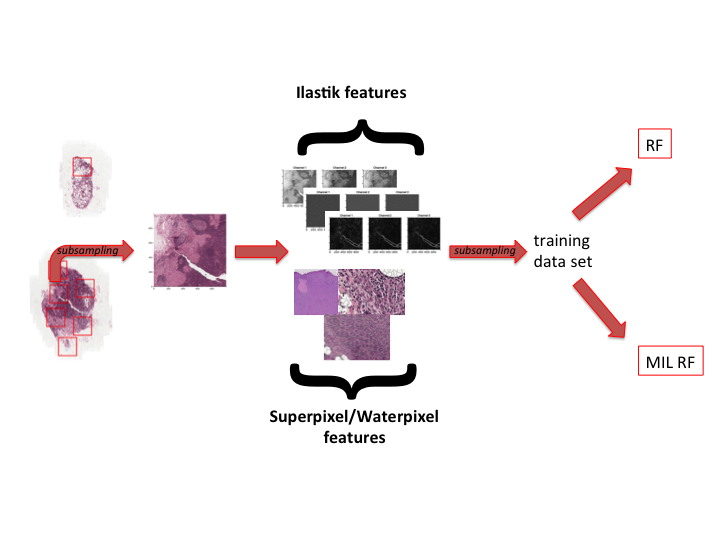
\includegraphics[width=0.9\textwidth]{workflow.png}
\caption{Camelyon2016 pipeline}
\label{Ol}
\end{figure}
\end{frame}

\begin{frame}{Ilastik}
\begin{columns}[T] % align columns
\begin{column}{.8\textwidth}

Ilastik : software for interactive image classification, segmentation and analysis. \\
Using features from ilastik (implemented in vigra, c++ library)
\begin{itemize}
\item Color/Intensity:
\begin{itemize}
\item [--] Gaussian Smoothing
\end{itemize}
\item Edge:
\begin{itemize}
\item [--] Laplacian of Gaussian
\item [--] Difference of Gaussians
\item [--] Gaussian Gradiant Magnitude
\end{itemize}
\item Texture:
\begin{itemize}
\item [--] Structure Tensor Eigenvalues
\item [--] Hessian of Gaussian Eigenvalues
\end{itemize}
\end{itemize}
\end{column}%
\begin{column}{.2\textwidth}
\begin{figure}[!ht]
\centering

\includegraphics[width=\textwidth]{Ilastik.png}
\caption{Ilastik}
\label{}
\end{figure}
\end{column}%
\end{columns}
\end{frame}


\begin{frame}{Pixel based classifier: outputs}

\begin{small}
\begin{figure}[!ht]
\centering
\begin{subfigure}{.3\textwidth}
  \centering
  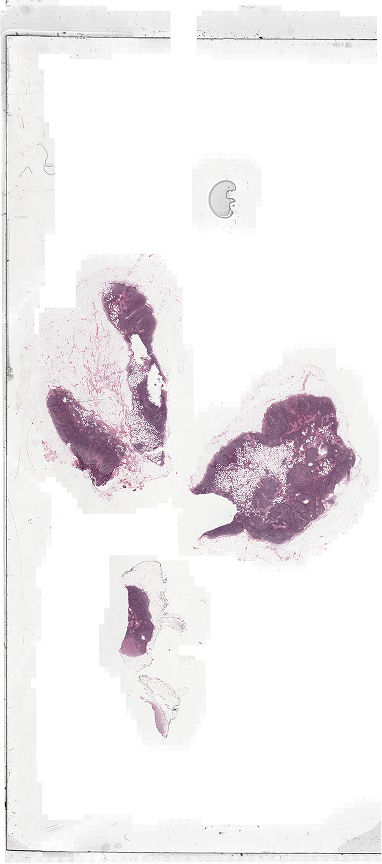
\includegraphics[width=\linewidth, height=5cm]{Test_002_whole.png}
  \caption{RGB raw data.}
  \label{RawImage}
\end{subfigure}%
\begin{subfigure}{.3\textwidth}
  \centering
  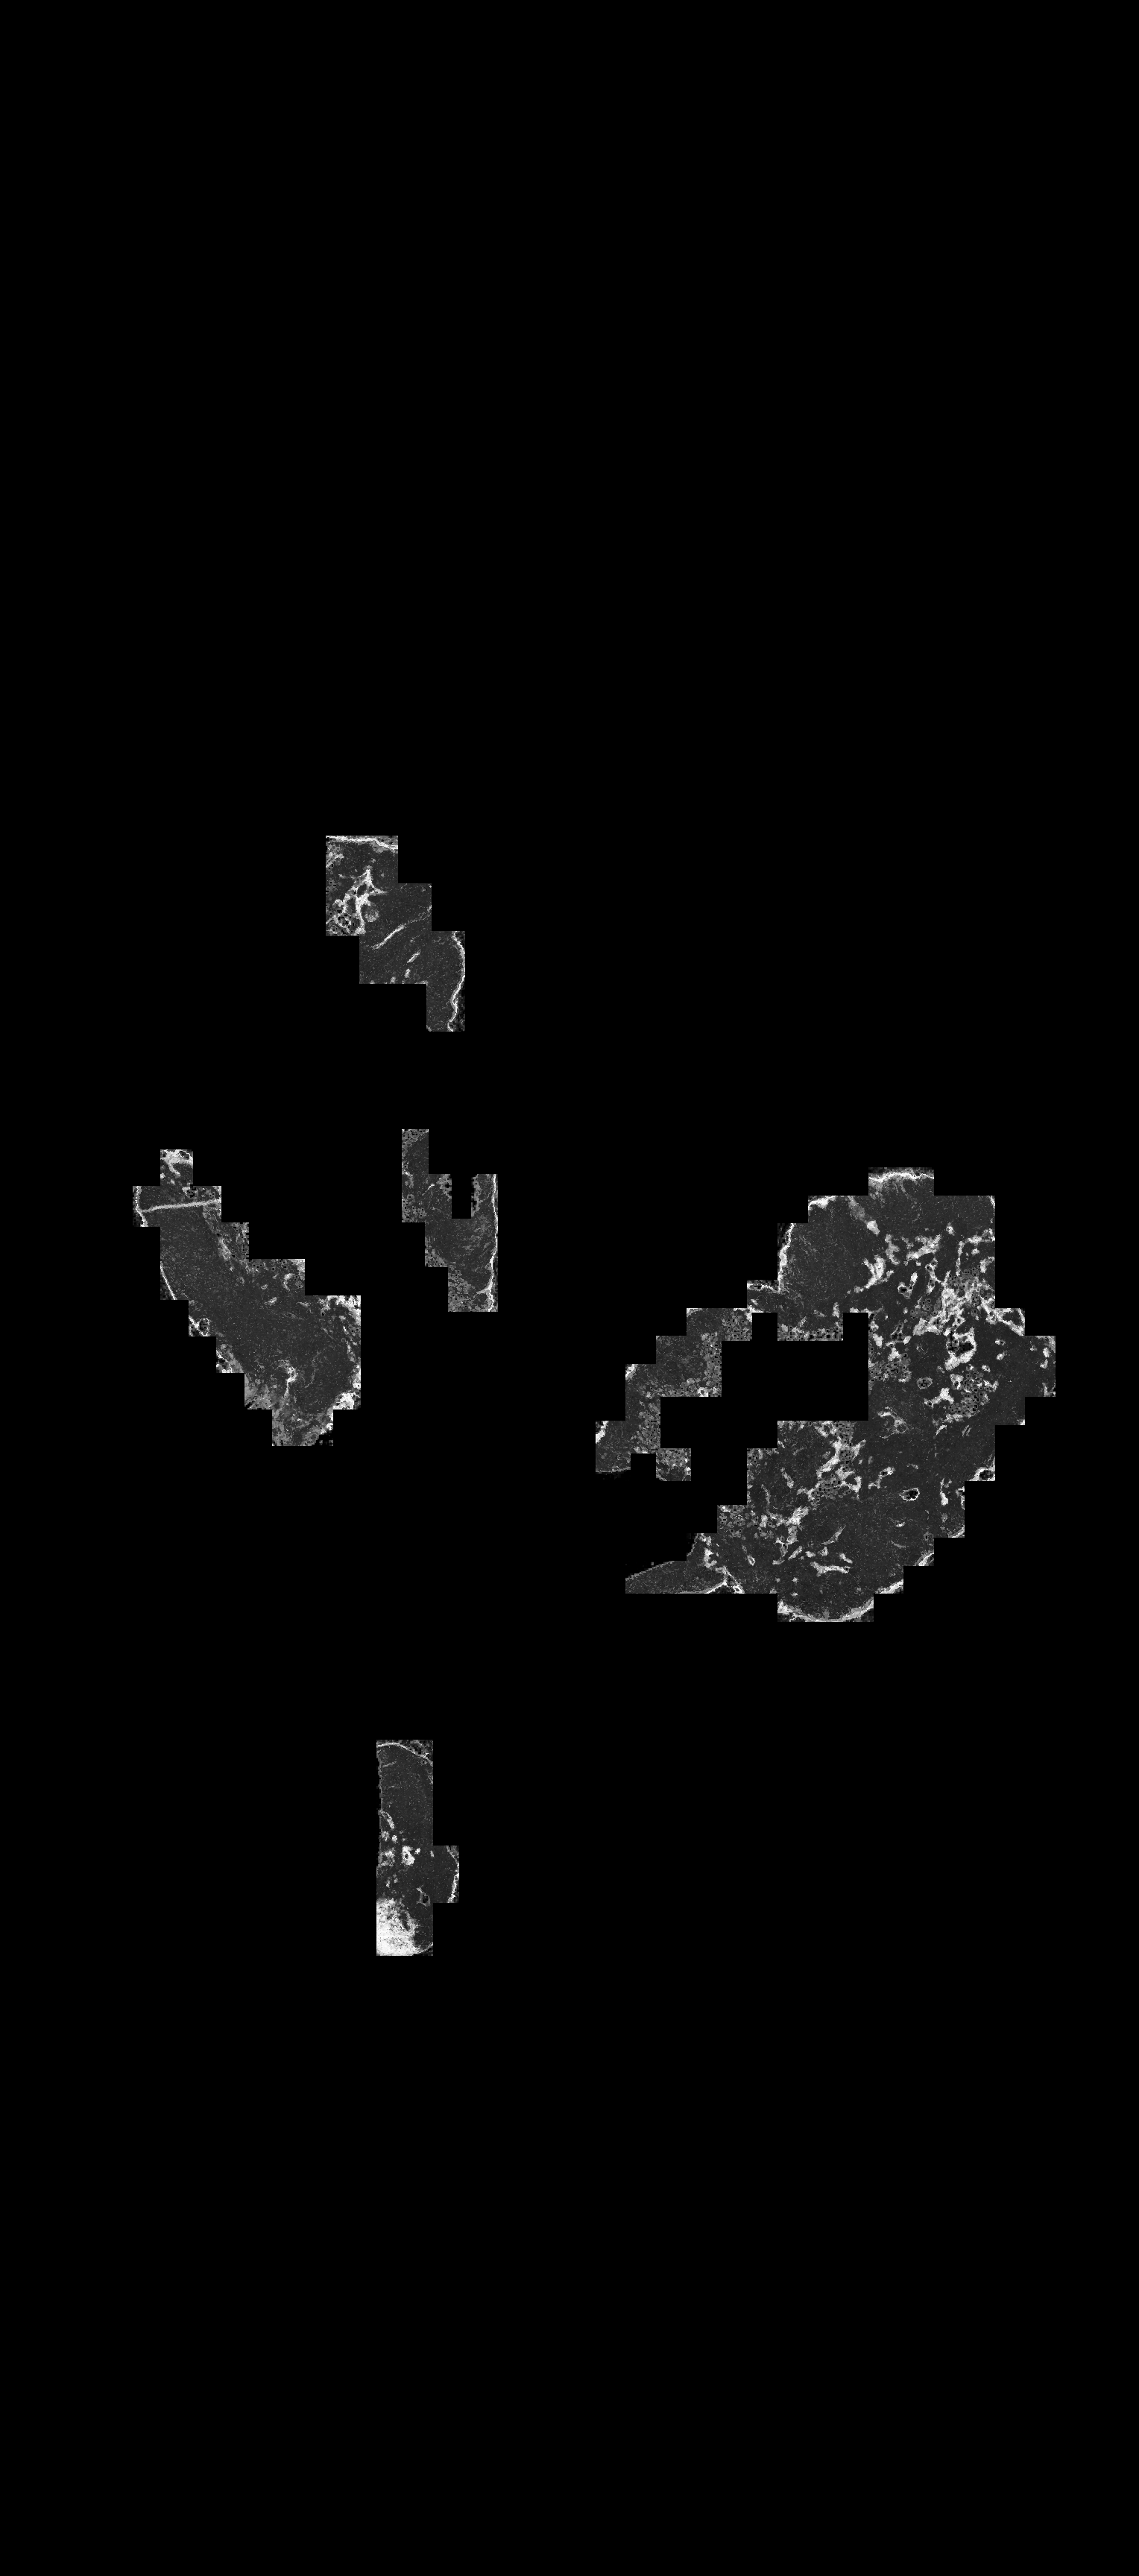
\includegraphics[width=\linewidth, height=5cm]{whole_probmap_Test_002.png}
  \caption{Probability map.}
  \label{ProbabilityMapLocalMaxima}
\end{subfigure}
\begin{subfigure}{.3\textwidth}
  \centering
  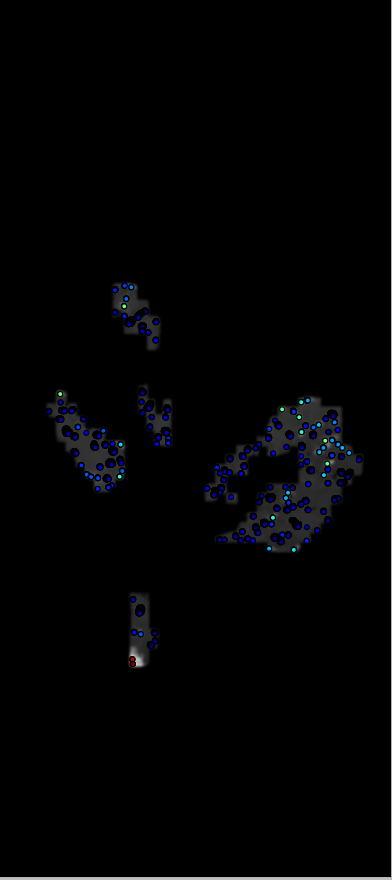
\includegraphics[width=\linewidth, height=5cm]{Detection.png}
  \caption{Prediction points.}
  \label{Detecting maxima}
\end{subfigure}
\\
\textit{For figure (c), blue is equal to a low confidence score whereas red means a high confidence.}
\caption{Evaluation whole slide image, test slide number 2.}

\label{fig:test}
\end{figure}
\end{small}
\end{frame}

\begin{frame}{Results and perspective}
\begin{itemize}
\item We had an AUC score of $0,63$.
\item Our features are based ilastik/waterpixels at different scales.
\item Unsufficient to predict the higlhly variable metastasis tissue.
\item Methods based on deep architecture achieved good performances.
\item Learning which features are relevant is the key point.
\item Next step: segmentation based on deep architecture, fully convolutionnal networks \footfullcite{long2015fcn}.
\end{itemize}
\end{frame}


\section{Current work}
%% I will talk about my current work + data F.Reyal
%% 6/7 slides approx

\begin{frame}{PhD pipeline}
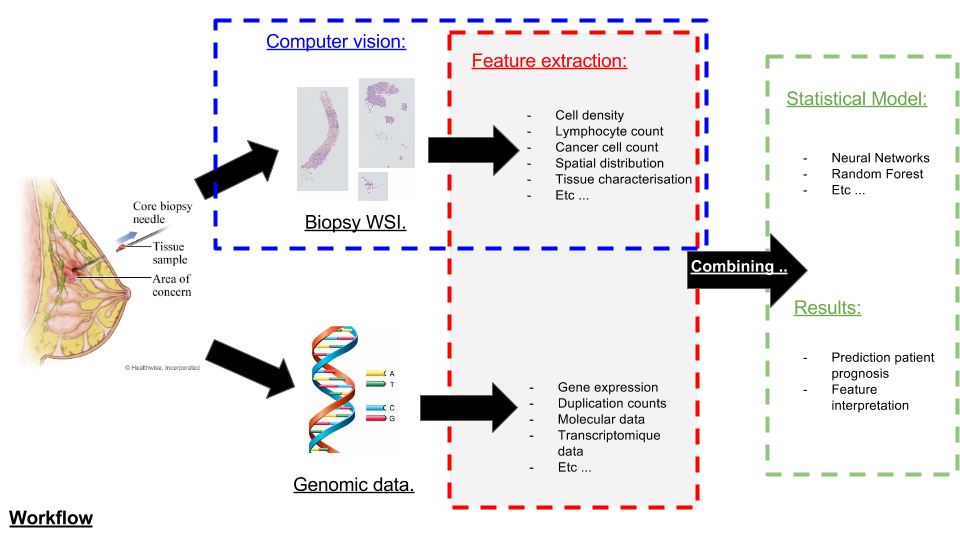
\includegraphics[width=\textwidth]{Workflow_overview.png}
\end{frame}
\begin{frame}{Computer Vision}
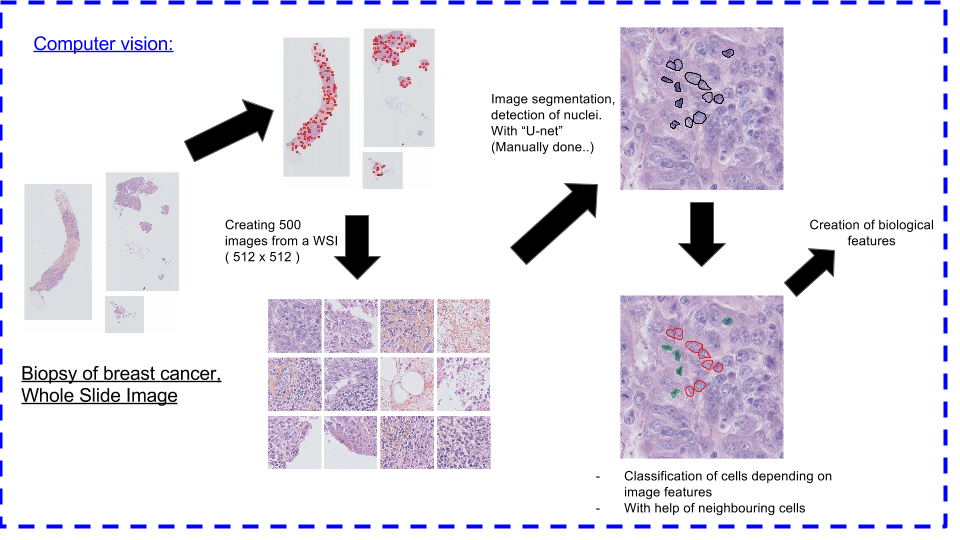
\includegraphics[width=\textwidth]{ComputerVision.png}
\end{frame}

\begin{frame}{Data}
Very similar data as Camelyon2016, but messier. 
We had to better segment the tissue area.
\begin{columns}[T] % align columns
\begin{column}{.5\textwidth}
\begin{figure}[!ht]
\centering
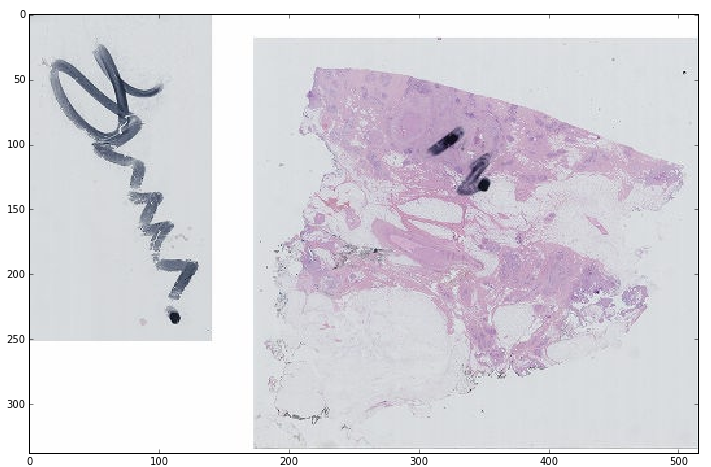
\includegraphics[width=0.9\textwidth]{slideFabien1.png}\par 
\caption{Whole slide tumor}
\label{fig: fab1}
\end{figure}
\end{column}%
\begin{column}{.5\textwidth}
\begin{figure}[!ht]
\centering
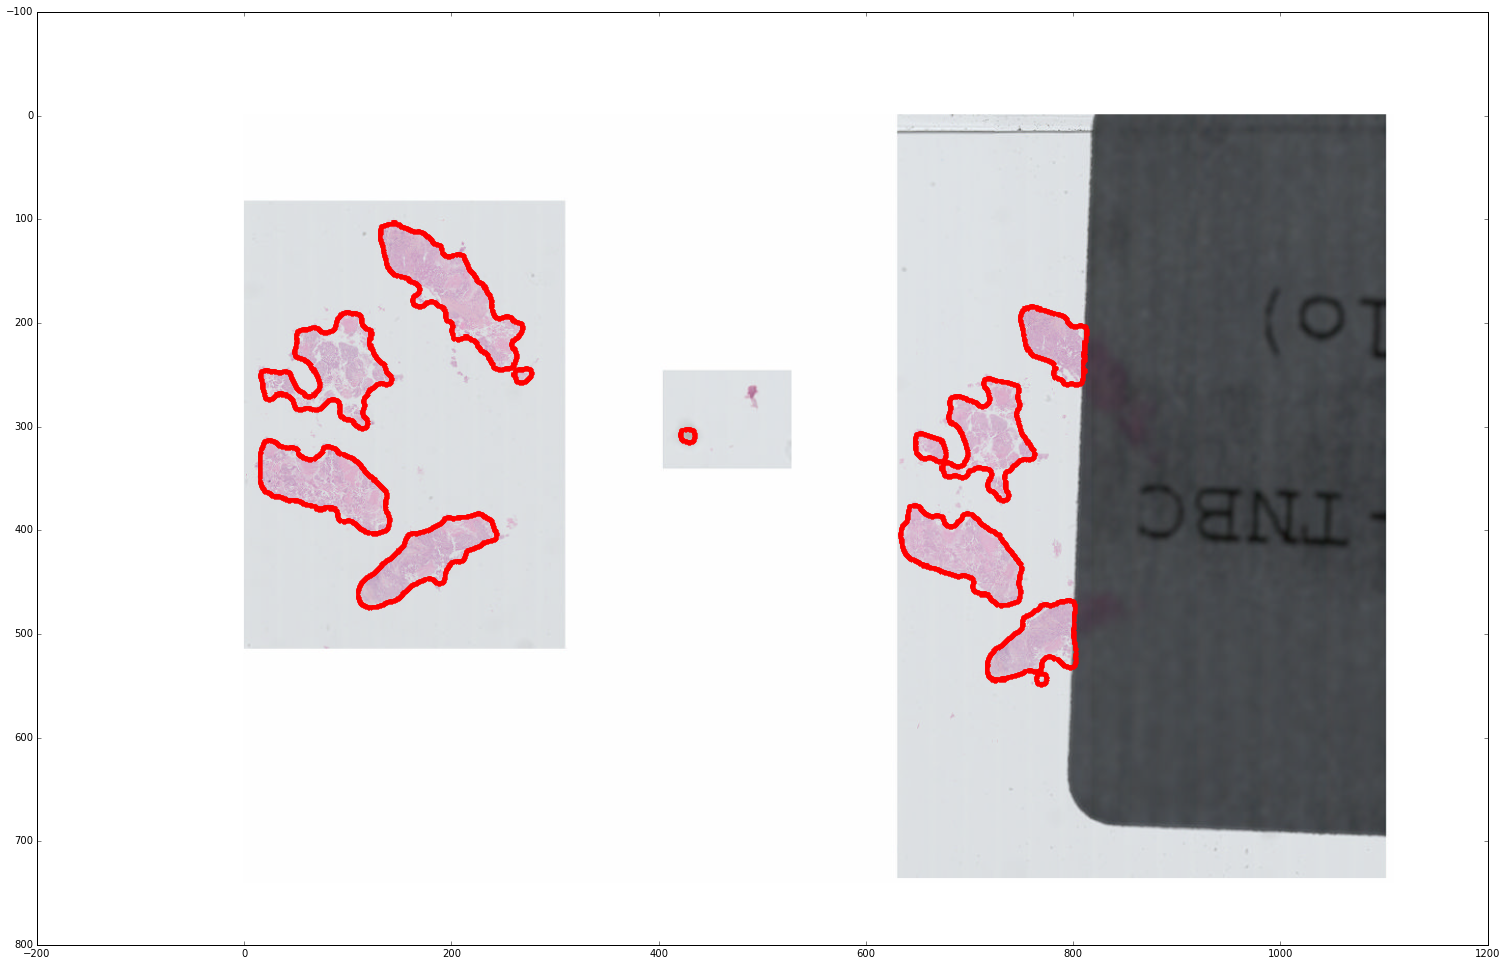
\includegraphics[width=0.9\textwidth]{slideFabien2.png}\par 
\caption{Biopsy}
\label{fig: fab2}
\end{figure}
\end{column}%
\end{columns}


\end{frame}


\begin{frame}{Annotations}
\begin{itemize}
\item Manual annotations at the cell/tissue level.
\item Issue very little ground truth while deep networks need a lot of data? Data augmentation! \\
\end{itemize}

\begin{columns}[T] % align columns
\begin{column}{.16\textwidth}
\begin{figure}[!ht]
\centering
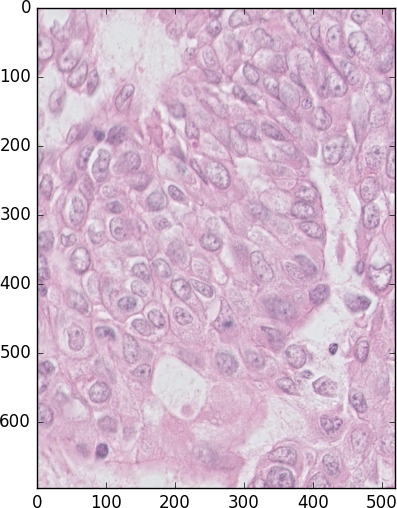
\includegraphics[width=0.9\textwidth]{BIS.png}\par 
\caption{Original}
\label{fig: ori}
\end{figure}
\end{column}%
\begin{column}{.16\textwidth}
\begin{figure}[!ht]
\centering
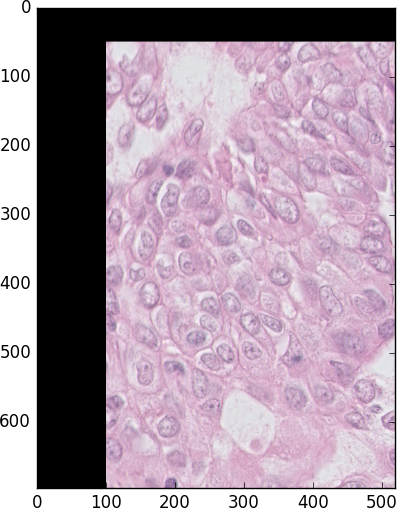
\includegraphics[width=0.9\textwidth]{shift.png}\par 
\caption{Translated}
\label{fig:shift}
\end{figure}
\end{column}%
\begin{column}{.16\textwidth}
\begin{figure}[!ht]
\centering
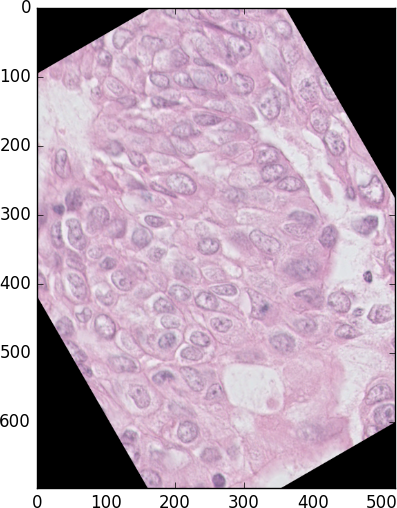
\includegraphics[width=0.9\textwidth]{rot.png}\par 
\caption{Rotated}
\label{fig:rot}
\end{figure}
\end{column}%
\begin{column}{.16\textwidth}
\begin{figure}[!ht]
\centering
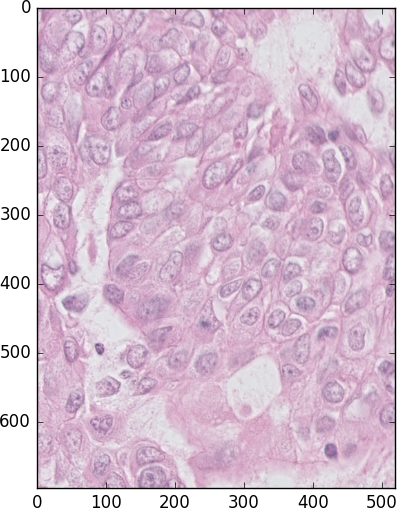
\includegraphics[width=0.9\textwidth]{flip.png}\par 
\caption{Flipped}
\label{fig: flip}
\end{figure}
\end{column}
\begin{column}{.16\textwidth}
\begin{figure}[!ht]
\centering
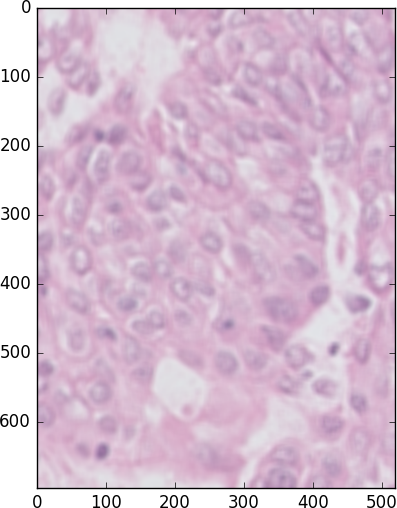
\includegraphics[width=0.9\textwidth]{blur.png}\par 
\caption{Blurred}
\label{fig: blur}
\end{figure}
\end{column}%
\begin{column}{.16\textwidth}
\begin{figure}[!ht]
\centering
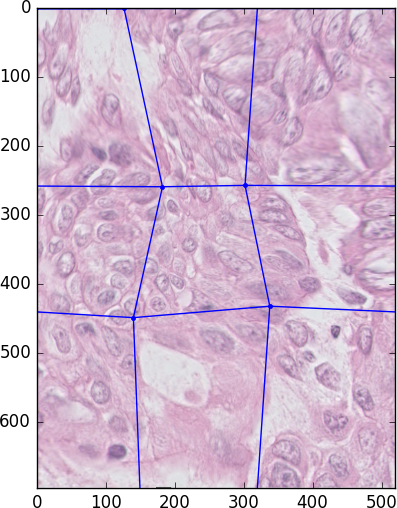
\includegraphics[width=0.9\textwidth]{ELAST.png}\par 
\caption{Elastic distortion}
\label{fig: Elastic distortions}
\end{figure}
\end{column}%

\end{columns}

Data augmentation can make the network learn the proper invariances! \footfullcite{UNet}.
%
%\begin{figure}
%\begin{multicols}{6}
%	\begin{subfigure}{0.2\textwidth}
%    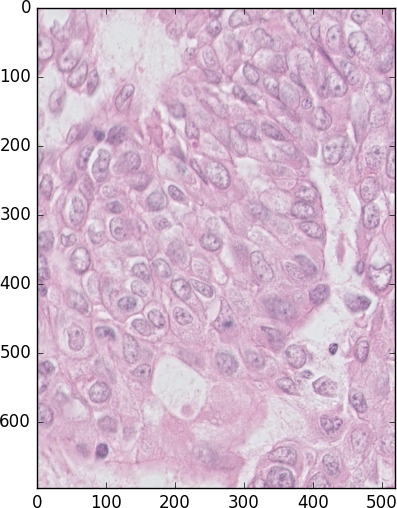
\includegraphics[width=0.9\textwidth]{BIS.png}\par 
%     \caption{Original image}
%     \label{fig:original}
%	\end{subfigure}%
%	\begin{subfigure}{0.2\textwidth}
%    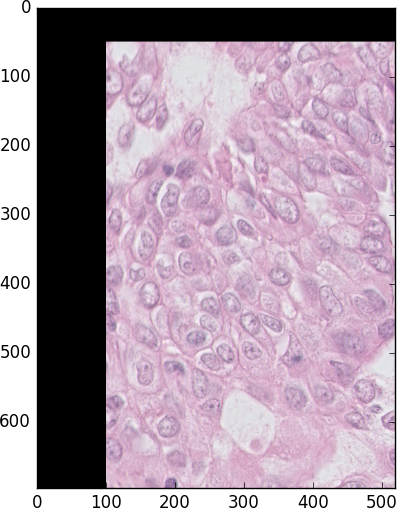
\includegraphics[width=0.9\textwidth]{shift.png}\par 
%    \caption{Translated}
%    \label{fig:shift}
%	\end{subfigure}%
%	\begin{subfigure}{0.2\textwidth}
%    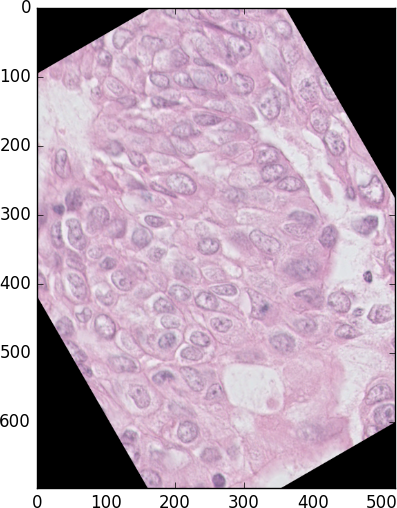
\includegraphics[width=0.9\textwidth]{rot.png}\par 
%     \caption{Rotated}
%     \label{fig:rot}
%	\end{subfigure}%
%    \begin{subfigure}{0.2\textwidth}
%    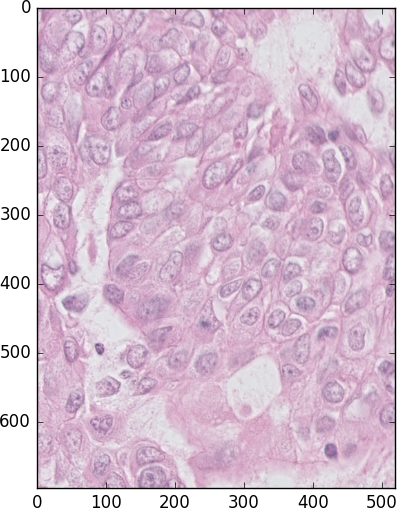
\includegraphics[width=0.9\textwidth]{flip.png}\par 
%     \caption{Vertical flip}
%     \label{fig:flip}
%	\end{subfigure}%
%	\begin{subfigure}{0.2\textwidth}
%    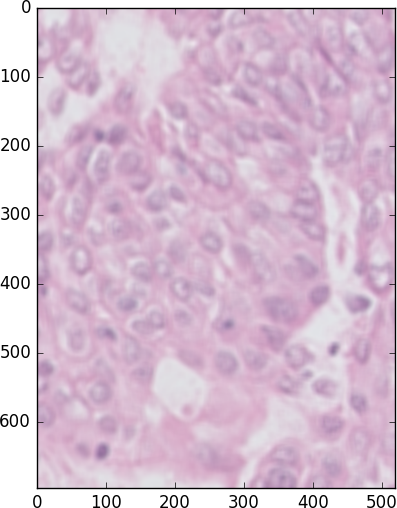
\includegraphics[width=0.9\textwidth]{blur.png}\par 
%    \caption{Out of focus}
%    \label{fig:blur}
%	\end{subfigure}%
%	\begin{subfigure}{0.2\textwidth}
%    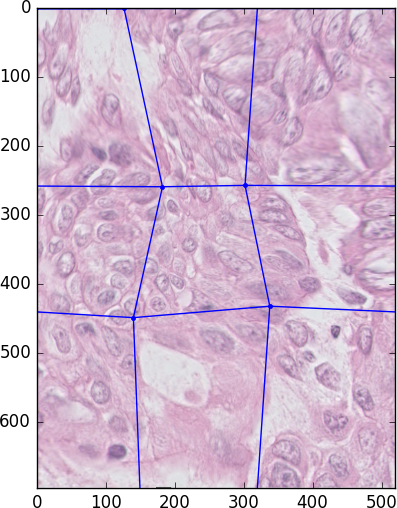
\includegraphics[width=0.9\textwidth]{ELAST.png}\par 
%     \caption{Elastic deformation}
%     \label{fig:elastic}
%	\end{subfigure}%
%\end{multicols}
%\caption{Data augmentation}
%\end{figure}

\end{frame}

\section{Github and Jupyter notebook}

\begin{frame}{Jupyter notebook and Github}
\url{https://github.com/PeterJackNaylor?tab=repositories}
\begin{figure}
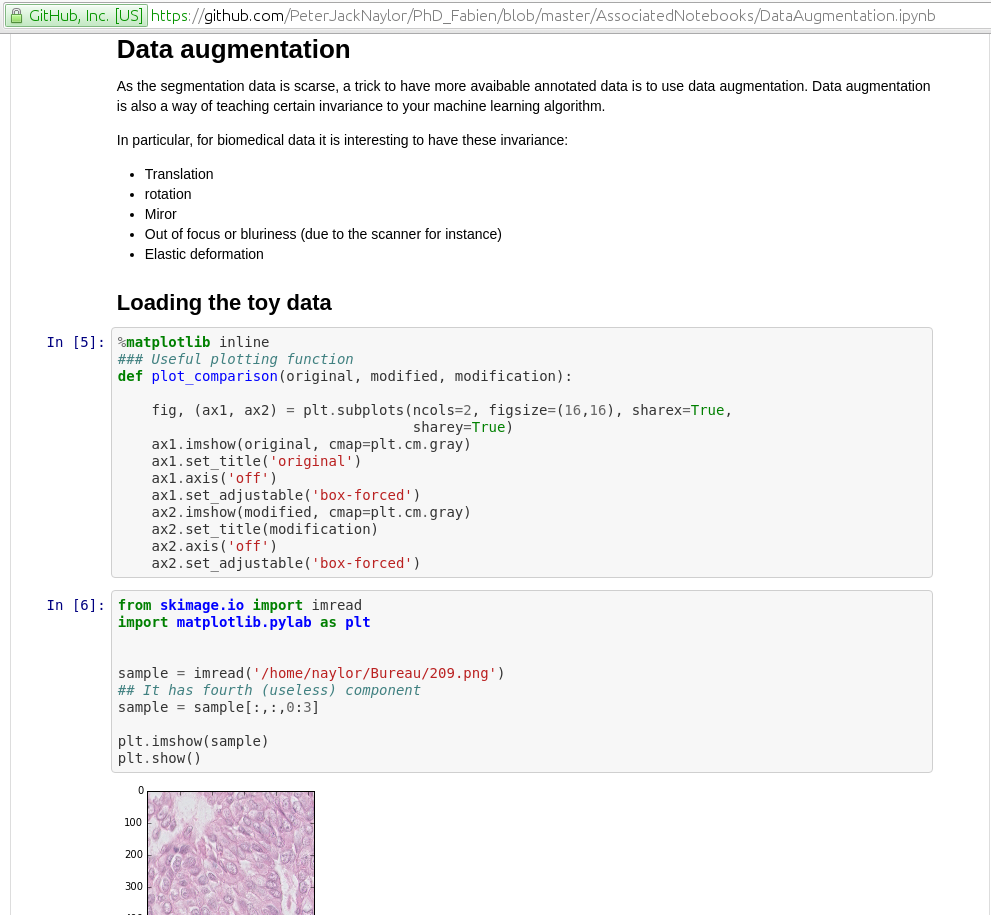
\includegraphics[width=0.8\textwidth]{GitBook.png}
\caption{Jupyter notebook and github}
\end{figure}
\end{frame}


\begin{frame}[noframenumbering]
The end! :-)
\end{frame}
\section*{Appendix}

\begin{frame}[noframenumbering]{Camelyon16}

\begin{columns}[T] % align columns
\begin{column}{.50\textwidth}
\begin{small}
\textcolor{red}{Goal:}
\begin{itemize}
\item Detection of micro- and macro-metastases in lymph node digitized images.
\item Automated detection of metatases in hematoxylin and eosin (H\&E) stained whole-slide images of lymph node sections.
\end{itemize}
\textcolor{red}{Motivation:}
\begin{itemize}
\item Lymph node metastases occur in most cancer types.
\item Lymph nodes in the underarm are the first place cancer is likely to spread.
\item The prognosis is poorer when cancer has spread there.
\end{itemize}
\end{small}
\end{column}%
\hfill%
\begin{column}{.50\textwidth}
\begin{figure}[!ht]
\centering
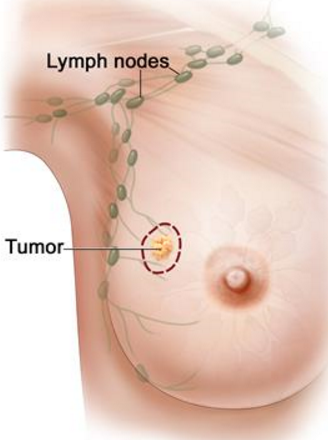
\includegraphics[width=\textwidth]{Booby.png}
\label{booby}
\end{figure}
\end{column}%
\end{columns}

\end{frame}

\begin{frame}[noframenumbering]{Camelyon16}

\begin{columns}[T] % align columns
\begin{column}{.50\textwidth}
\begin{small}
\textcolor{red}{Goal:}
\begin{itemize}
\item Detection of micro- and macro-metastases in lymph node digitized images.
\item Automated detection of metastases in hematoxylin and eosin (H\&E) stained whole-slide images of lymph node sections.
\end{itemize}
\end{small}
\begin{figure}[!ht]
\centering
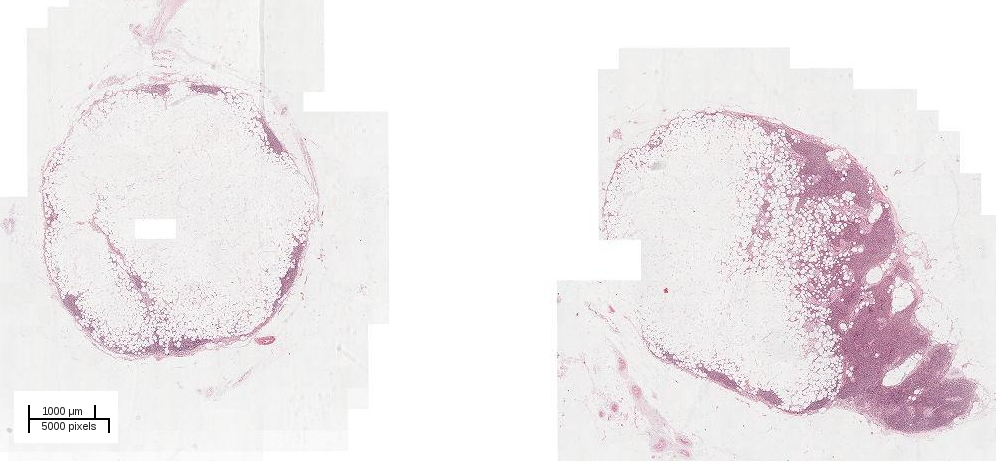
\includegraphics[width=\textwidth]{Normal_38.png}
\caption{Normal 38}
\label{normal_38}
\end{figure}
\end{column}%
\hfill%
\begin{column}{.50\textwidth}
\begin{figure}[!ht]
\centering
\includegraphics[width=\textwidth]{Tumor_34.png}
\caption{Tumor 34}
{\footnotesize \textit{Metastases detected in green}}
\label{tumor_34}
\end{figure}
\end{column}%
\end{columns}

\end{frame}

% You can reveal the parts of a slide one at a time
% with the \pause command:
\begin{frame}[noframenumbering]{Evaluation}
Two evaluation metrics and two leader boards. \\
\textcolor{red}{Slides based:}
\begin{itemize}
\item Binary classification of whether or not a slide contains metastases. \item Evaluating with the area under the ROC curve. 
%\item Model:  Multiple Instance Learning models, with a random forest or support vector machine.
\end{itemize}
\textcolor{red}{Region based:}
\begin{itemize}
\item Correctly detecting metastases within slides.
\item Evaluation with the FROC curve (free-response receiver operating characteristic)
%\item Pixel binary classification where a pixel will be labelled "Metastasis" if this pixel belongs to a metastasis.
\end{itemize}
\end{frame}

\begin{frame}[noframenumbering]{The data set}
\begin{columns}[T] % align columns
\begin{column}{.5\textwidth}
Data set provided:
\begin{itemize}
\item 160 Normal slides.
\item 110 Tumor slides.
\end{itemize} 

\begin{small}

\begin{itemize}
\item [--] Huge images with very high precisions, using c++ library openslide. 
\item [--] One image compressed with JPEG2000: $\sim$ 2/3Gb. 
\item [--] Uncompressed at approx. 10Gb. 
\item [--] Highest resolution : $\sim 96 256\times 218624$.
\item [--] Lowest resolution : $\sim 188 \times 427$. 
\end{itemize}
\end{small}

\end{column}%
\hfill%
\begin{column}{.5\textwidth}
\begin{figure}[!ht]
\centering
\includegraphics[width=\textwidth]{pyramid.png}
\caption{Pyramid data structure}
\textit{Between 8 and 10 different resolutions}
\label{}
\end{figure}
\end{column}%
\end{columns}

\end{frame}


\begin{frame}[noframenumbering]{Images}
\textcolor{red}{Very large number of samples:}
\begin{itemize}
\item In pixel classification, each pixel is an instance, n $\gg$ p.
\item Appropriate subsampling methods. In particular here, first subsampling for the "sub-images". Second subsampling given a particular "sub-image".
\end{itemize}
\end{frame}


\begin{frame}[noframenumbering]{Subsampling 1}
\textcolor{red}{Subsampling 1} (region of interest detection over slides)
Trying to find interesting part of the image. \\
We can divide sub-images in 4 groups.
\begin{itemize}
\item Only metastasis tissue.
\item Only normal tissue.
\item Centered on the boarder metastasis tissue/normal tissue.
\item Centered on the boarder tissue/background.
\end{itemize}
\end{frame}

\begin{frame}[noframenumbering]{Subsampling}

\begin{columns}[T] % align columns
\begin{column}{.25\textwidth}
\begin{figure}[!ht]
\centering
\includegraphics[width=\textwidth]{OnlyPositive.png}
\caption{Only metastasis regions}
\label{}
\end{figure}
\end{column}%
\begin{column}{.25\textwidth}
\begin{figure}[!ht]
\centering
\includegraphics[width=\textwidth]{OnlyNormal.png}
\caption{Only metastasis-free regions}
\label{}
\end{figure}
\end{column}%
\begin{column}{.25\textwidth}
\begin{figure}[!ht]
\centering
\includegraphics[width=\textwidth]{GT.png}
\caption{Ground truth}
\label{}
\end{figure}
\end{column}%
\begin{column}{.25\textwidth}
\begin{figure}[!ht]
\centering
\includegraphics[width=\textwidth]{Grid.png}
\caption{Grid partition}
\label{}
\end{figure}
\end{column}%
\end{columns}
\end{frame}

\begin{frame}[noframenumbering]{Ilastik - examples}
\begin{columns}[T] % align columns
\begin{column}{.8\textwidth}
\begin{figure}[!ht]
\centering
\includegraphics[width=.7\textwidth]{part3_sub1.png}
\caption{Gaussian smoothing, $\sigma=0.7$}
\label{}
\end{figure}
\begin{figure}[!ht]
\centering
\includegraphics[width=.7\textwidth]{part3_sub2.png}
\caption{Laplacian of Gaussian, $\sigma=5$}
\label{}
\end{figure}
\end{column}%
\begin{column}{.2\textwidth}
\begin{figure}[!ht]
\centering
\includegraphics[width=\textwidth]{Ilastik.png}
\caption{Ilastik}
\label{}
\end{figure}
\end{column}%
\end{columns}
\end{frame}

\begin{frame}[noframenumbering]{Waterpixels - examples}
\begin{columns}[T] % align columns

\begin{column}{.3\textwidth}
\begin{figure}[!ht]
\centering
\includegraphics[width=\textwidth]{waterpix_res0.png}
\caption{Waterpixels at resolution 0}
\label{}
\end{figure}
\end{column}%

\begin{column}{.3\textwidth}
\begin{figure}[!ht]
\centering
\includegraphics[width=\textwidth]{waterpix_res2.png}
\caption{Waterpixels at resolution 2}
\label{}
\end{figure}
\end{column}%

\begin{column}{.3\textwidth}
\begin{figure}[!ht]
\centering
\includegraphics[width=\textwidth]{waterpix_res4.png}
\caption{Waterpixels at resolution 4}
\label{}
\end{figure}
\end{column}%

\end{columns}
\end{frame}

\begin{frame}[noframenumbering]{Subsampling 2}
\textcolor{red}{Pixel classification}. \\
Still very large data-set. \\
260 slides $\rightarrow$ 100 sub-images per slides $\rightarrow$ 1 000 000 pixels per sub-images. \\
Need for a second resampling. \\
Resampling randomly? smartly, via unsupervised methods? K means algorithm? 
\end{frame}

\begin{frame}[noframenumbering]{Pixel based classifier}
\textcolor{red}{Finding metastasis regions:}\\
Each pixel, will be considered metastasis if it belongs to a metastasis region. \\
Model: random forest. \\
\textcolor{red}{Detecting metastasis patients:}
Each pixel is or not a metastasis but it also belongs to bigger group. This larger group, the slide, is annotated. \\
Model: Multiple instance learning random forest.
\textcolor{red}{Cross-validation/evaluation:} \\
One slide out scheme.
\end{frame}

\begin{frame}[noframenumbering]{Multiple instance learning}
\textcolor{red}{Notations}:
\begin{itemize}
\item Pixels are a pair $(x_i,y_i) \in \mathbb{R}^d \times \lbrace -1, +1\rbrace$.
\item Slides are bags of pixels: $B_I=\lbrace x_i, i\in I \rbrace$, and we have $Y_I=1$ if there is at least one $x_i$ in $B_I$ that is positive, otherwise $Y_I=-1$. 
\item \textcolor{red}{Constraint to add} to an optimization problems: \\
$$\sum \frac{y_i+1}{2} \geqslant 1, \forall I \ s.t \ Y_I=1 \ \text{and} \ y_i=-1, \forall I \ s.t \ Y_I=-1$$
\end{itemize}
\textcolor{green}{Implementation} : MISVM, Multiple-Instance Support Vector Machines by Gary Doran. Python package. \\
\textcolor{green}{Paper}: \textit{Support Vector Machines for Multiple Instance learning}, S. Andrews, I. Tsochantaridis and T. Hofmann.
\end{frame}


\begin{frame}[noframenumbering]{Superpixels/Waterpixels}
Superpixels: Regions resulting from a low-level segmentation. 
They have these proprieties: \textcolor{red}{homogeneity, connected partitions, adherence to object boundaries, regularity}.
\begin{figure}[!ht]
\centering
\includegraphics[width=\textwidth]{Waterpixels.png}
\caption{Illustration of how superpixels are used}
\label{}
\end{figure}
\begin{small}
For more details \footfullcite{waterpixels}.
\end{small}
\end{frame}


\begin{frame}[noframenumbering]{Challenge results}
We did a score of 22nd out of 23. \\
Only three teams performed non-deep convolutionnal network. We were 2nd among these 3 teams.
\begin{figure}[!ht]
\centering
\includegraphics[width=0.5\textwidth]{ROC.png}
\caption{ROC curve associated to the slide base evaluation}
\label{Eval: ROC}
\end{figure}
\end{frame}

\end{document}


